\documentclass[11pt]{article}
%\usepackage{fullpage,graphicx,algorithm,algorithmic,bm,amsmath,amsthm,amssymb,color,hyperref,cite,natbib}

% if you need to pass options to natbib, use, e.g.:
%\PassOptionsToPackage{numbers}{natbib}
\usepackage{natbib,fullpage}
\usepackage{bm,amsmath,amsthm,amssymb,multicol,algorithmic,algorithm,enumitem}
\usepackage{wrapfig,lipsum}
\usepackage[textwidth=1cm,textsize=footnotesize]{todonotes}

% ready for submission
\usepackage{neurips_2020}

\usepackage[colorlinks=true,
linkcolor=red,
urlcolor=blue,
citecolor=blue]{hyperref}
\usepackage{hyperref}
\usepackage{cleveref}

\setlength{\parskip}{.2cm}

\newtheorem{Fact}{Fact}
\newtheorem{Lemma}{Lemma}
\newtheorem{Prop}{Proposition}
\newtheorem{Theorem}{Theorem}
\newtheorem{Def}{Definition}
\newtheorem{Corollary}{Corollary}
\newtheorem{Conjecture}{Conjecture}
\newtheorem{Property}{Property}
\newtheorem{Observation}{Observation}
%\theorembodyfont{\rmfamily}
\newtheorem{Exa}{Example}
\newtheorem{assumption}{H\!\!}
\newtheorem{assumptionA}{S\!\!}
\newtheorem{assumptionL}{L\!\!}
\newtheorem{Remark}{Remark}
\newtheorem*{Lemma*}{Lemma}
\newtheorem*{Theorem*}{Theorem}
 \makeatletter
\renewenvironment{proof}[1][\proofname]{%
   \par\pushQED{\qed}\normalfont%
   \topsep6\p@\@plus6\p@\relax
   \trivlist\item[\hskip\labelsep\bfseries#1]%
   \ignorespaces
}{%
   \popQED\endtrivlist\@endpefalse
}
\makeatother

%%%%%%%%%%% Stuffs for Tikz %%%%%%%%%%%%%%%%%%
\usepackage{pgfplots}
\usepackage{xargs}
\usepackage{stmaryrd}
\usetikzlibrary{arrows,shapes,calc,tikzmark,backgrounds,matrix,decorations.markings}
\usepgfplotslibrary{fillbetween}
\pgfplotsset{compat=1.3}
\usepackage{subfig}

\usepackage{relsize}
\tikzset{fontscale/.style = {font=\relsize{#1}}
    }

\definecolor{lavander}{cmyk}{0,0.48,0,0}
\definecolor{violet}{cmyk}{0.79,0.88,0,0}
\definecolor{burntorange}{cmyk}{0,0.52,1,0}

\def\lav{lavander!90}
\def\oran{orange!30}

\definecolor{asuorange}{rgb}{1,0.699,0.0625}
\definecolor{asured}{rgb}{0.598,0,0.199}
\definecolor{asuborder}{rgb}{0.953,0.484,0}
\definecolor{asugrey}{rgb}{0.309,0.332,0.340}
\definecolor{asublue}{rgb}{0,0.555,0.836}
\definecolor{asugold}{rgb}{1,0.777,0.008}

%%%%%%%%%%%%%%%%%%%%%%%%%%%%%%%%%%%%%


\usepackage{shortcuts_OPT}

%\renewcommand{\textwidth}{5.5in}

% Here's the definition of Sb, stolen from amstex
    \makeatletter
    \def\multilimits@{\bgroup
  \Let@
  \restore@math@cr
  \default@tag
 \baselineskip\fontdimen10 \scriptfont\tw@
 \advance\baselineskip\fontdimen12 \scriptfont\tw@
 \lineskip\thr@@\fontdimen8 \scriptfont\thr@@
 \lineskiplimit\lineskip
 \vbox\bgroup\ialign\bgroup\hfil$\m@th\scriptstyle{##}$\hfil\crcr}
    \def\Sb{_\multilimits@}
    \def\endSb{\crcr\egroup\egroup\egroup}
\makeatother

\newtheoremstyle{t}         %name
    {\baselineskip}{2\topsep}      %space above and below
    {\rm}                   %Body font
    {0pt}{\bfseries}  %Heading indent and font
    {}                      %after heading
    { }                      %head after space
    {\thmname{#1}\thmnumber{#2}.}

\theoremstyle{t}
\newtheorem{q}{Q}
\parindent=0pt

%\newcommand{\eric}[1]{\todo[color=red!20]{{\bf EM:} #1}}
%\newcommand{\erici}[1]{\todo[color=red!20,inline]{{\bf EM:} #1}}
%\newcommand{\belhal}[1]{\todo[color=green!20]{{\bf BK:} #1}}
%\newcommand{\belhali}[1]{\todo[color=green!20,inline]{{\bf BK:} #1}}
%\newcommand{\toco}[1]{\todo[color=yellow!20]{{\bf To:} #1}}



\makeatletter
\DeclareRobustCommand*\cal{\@fontswitch\relax\mathcal}
\makeatother

\begin{document}
\title{\vspace{-0.1in}MISSO: Minimization by Incremental Stochastic Surrogate Optimization for Large Scale Nonconvex and Nonsmooth Problems\vspace{-0.1in}}

\author{
  Belhal Karimi \\
  Cognitive And Computing Lab\\
  Baidu Research\\
  Beijing, China \\
  \texttt{belhal.karimi@baidu.com} 
   \And
   Hoi-To Wai \\
   Department of SEEM\\
   The Chinese University of Hong Kong\\
   Hong Kong \\
   \texttt{htwai@se.cuhk.edu.hk} \\
   \And
   Eric Moulines \\
   Center of Applied Mathematics\\
   Ecole Polytechnique\\
   Palaiseau, FR \\
   \texttt{eric.moulines@polytechnique.fr} \\
   \And
  Ping Li \\
  Cognitive And Computing Lab\\
  Baidu Research\\
  Beijing, China \\
  \texttt{liping@baidu.com} \\
}

\date{\today}

\maketitle

\begin{abstract}\vspace{-0.1in}
Many constrained, non-convex optimization problems can be tackled using the Majorization-Minimization (MM) method which alternates between constructing a surrogate function which upper bounds the objective function, and then minimizing this surrogate.
For problems which minimize a finite sum of functions, a stochastic version of the MM method selects a batch of functions at random at each iteration and optimizes the accumulated surrogate.
However, in many cases of interest such as  variational inference for latent variable models, the surrogate functions are expressed as an expectation. In this contribution, we propose a doubly stochastic MM method based on Monte Carlo approximation of these stochastic surrogates.
We establish asymptotic and non-asymptotic convergence of our scheme in a constrained, non-convex, non-smooth optimization setting.
We apply our new framework for inference of logistic regression model with missing covariates and for variational inference of Bayesian variants of LeNet-5 and Resnet-18 on respectively the MNIST and CIFAR-10 datasets.
\end{abstract}

\vspace{-0.1in}
\section{Introduction}
\vspace{-0.05in}

We consider the \emph{constrained} minimization problem of a finite sum of  functions:
\beq \label{eq:opt}
\min_{ \param \in \Param }~ {\cal L} ( \param ) \eqdef \frac{1}{n} \sum_{i=1}^n {\cal L}_i( \param) \eqsp,
\eeq
where $\Theta$ is a convex, compact, and closed subset of $\rset^p$, and for any $i \in \inter$, the function ${\cal L} _i: \rset^p \to \rset$ is bounded from below and is (possibly) non-convex and non-smooth.

To tackle the optimization problem \eqref{eq:opt}, a popular approach is to apply the majorization-minimization (MM) method which iteratively minimizes a majorizing surrogate function. A large number of existing procedures fall into this general framework, for instance gradient-based or proximal methods or  the Expectation-Maximization (EM) algorithm \citep{mcLachlan2008em} and some variational Bayes inference techniques \citep{jordan1999var}; see for example \citep{razaviyayn2013unified} and \citep{lange2016mm} and the references therein.
When the number of terms $n$ in \eqref{eq:opt} is large, the vanilla MM method may  be intractable because it requires to construct a surrogate function for all the $n$ terms ${\cal L}_i$ at each iteration. Here, a remedy is to apply the Minimization by Incremental Surrogate Optimization (MISO) method proposed by \citet{mairal2015miso}, where the surrogate functions are updated incrementally. The MISO method can be interpreted as a combination of MM and ideas which have emerged for variance reduction in stochastic gradient methods \citep{schmidt2017minimizing}.
An extended analysis of MISO in both the convex and nonconvex case has resently been proposed in \citep{qian2019miso}.

The success of the MISO method rests upon the efficient minimization of surrogates such as convex functions, see \citep[Section 2.3]{mairal2015miso}. In many applications of interest, the natural surrogate functions are intractable, yet they are  defined as expectation of tractable functions. This for example the case for inference in latent variable models. Another application is variational inference, \citep{ghahramani2015probabilistic}, in which  the goal is to approximate the posterior distribution of parameters given the observations;  see for example \citep{neal2012bayesian,blundell2015weight,polson2017deep,rezende2014stochastic, li2017dropout}.


This paper fills the gap in the literature by proposing a new method called \emph{Minimization by Incremental Stochastic Surrogate Optimization (MISSO)} which is designed for the finite sum optimization with a finite-time convergence guarantee.
Our contributions can be summarized as follows.
\begin{itemize}
\item We propose a unifying framework of analysis for incremental stochastic surrogate optimization when the surrogates are defined by expectations of tractable functions. The proposed  MISSO method is built on the Monte Carlo integration of the intractable surrogate function, \ie a doubly stochastic surrogate optimization scheme.
\item We present an incremental update of the commonly used variational inference and Monte-Carlo EM methods as special cases of our newly introduced framework. The analysis of those two algorithms is thus done under this unifying framework of analysis.
\item We establish both asymptotic and non-asymptotic convergence for the  MISSO method. In particular, the MISSO method converges almost surely to a stationary point and in ${\cal O} (n/\epsilon)$ iterations to an $\epsilon$-stationary point.
\end{itemize}

In Section \ref{sec:framework}, we review the techniques for incremental minimization of finite sum functions based on the MM principle; specifically, we review the MISO method as introduced in \citep{mairal2015miso}, and present a class of  surrogate functions expressed as an expectation over a latent space. 
The MISSO method is then introduced for the latter class of intractable surrogate functions requiring approximation.
In Section \ref{sec:analysis}, we provide the asymptotic and non-asymptotic convergence analysis for the MISSO method (and of the MISO \citep{mairal2015miso} one as a special case).
Finally, Section \ref{sec:numerical} presents numerical applications to illustrate our findings including parameter inference for logistic regression with missing covariates and variational inference for two types of Bayesian neural networks.

\textbf{Notations.}
We denote $\inter=\{1,\dots,n\}$. Unless otherwise specified,  $\| \cdot \|$ denotes the standard Euclidean norm and $\pscal{ \cdot }{\cdot }$ is the inner product in Euclidean space.
For any function $f : \Param \rightarrow \rset$,  $f'( \param, {\bm d} )$ is the directional derivative of $f$ at $\param$ along the direction ${\bm d}$, \ie
\beq
f'( \param, {\bm d} ) \eqdef \lim_{ t \rightarrow 0^+ } \frac{ f ( \param + t {\bm d} ) - f( \param ) }{ t } \eqsp.
\eeq
The directional derivative is assumed to exist for the functions introduced throughout this paper.


\vspace{-0.05in}
\section{Incremental Minimization of Finite Sum Non-convex Functions}\label{sec:framework}
\vspace{-0.05in}

The objective function in \eqref{eq:opt} is composed of a finite sum of possibly non-smooth and non-convex functions.
A popular approach here is to apply the MM method. The MM method tackles \eqref{eq:opt} through alternating between two steps --- {\sf (i)} minimizing a  \emph{surrogate} function which upper bounds the original objective function; and {\sf (ii)} updating the surrogate function to tighten the upper bound.

As mentioned in the Introduction, the MISO method proposed by \citet{mairal2015miso} is developed as an iterative scheme that only  updates the surrogate functions \emph{partially} at each iteration.
Formally, for any $i \in \inter$, we consider a surrogate function $\sur{i}{\param}{\op}$ which satisfies
\begin{assumptionA} \label{ass:sur} For all $i \in \inter$ and $\op \in \Param$, the function $\sur{i}{\param}{\op}$ is convex \wrt $\param$, and it holds
\beq \label{eq:lowerbd}
\sur{i}{\param}{\op} \geq {\cal L}_i( \param ),~\forall~\param \in \Param \eqsp,
\eeq
where the equality holds when $\param = \op$.
\end{assumptionA}
\begin{assumptionA} \label{ass:diff}
For any $\op_i \in \Param$, $i \in \inter$ and some $\epsilon > 0$, the difference function $\widehat{e}(\param ; \{ \op_i \}_{i=1}^n ) \eqdef \frac{1}{n} \sum_{i=1}^n \sur{i}{\param}{\op_i } - {\cal L}( \param)$ is defined for all $\param \in \Param_\epsilon$ and differentiable for all $\param \in \Param$, where $\Param_\epsilon = \{ \param \in \rset^d, \inf_{\param' \in \Param} \| \param - \param' \| < \epsilon \}$ is an $\epsilon$-neighborhood set of $\Param$. Moreover, for some constant $L$, the gradient satisfies
\beq
\label{eq:eq30}
\| \grd \widehat{e}(\param; \{ \op_i \}_{i=1}^n)  \|^2 \leq 2 L\!~ \widehat{e}(\param; \{ \op_i \}_{i=1}^n) ,~\forall~\param \in \Param \eqsp.
\eeq
\end{assumptionA}
%We remark that S\ref{ass:sur} is a common condition used for surrogate functions, see \citep[Section 2.3]{mairal2015miso}.
%Note that by \citep[Proposition 1]{razaviyayn2013unified},
S\ref{ass:sur} is a common condition used for surrogate optimization, see \citep[Section 2.3]{mairal2015miso}. Meanwhile, S\ref{ass:diff} can be satisfied when the difference function
$\widehat{e}(\param ; \{ \op_i \}_{i=1}^n )$ is $L$-smooth for all $\param \in \rset^d$, where the condition can be implied through applying \citep[Proposition 1]{razaviyayn2013unified}.
%Lastly, in practice in inference with missing data, the differentiability condition in S\ref{ass:diff} can be satisfied by taking $\Param$ to be a slightly smaller set than the admissible set in the distribution parameters.

% implies that
%$\widehat{\cal L}_i' (\op; \op, {\bm d} ) = {\cal L}_i' ( \op, {\bm d} )$ for all ${\bm d}$ such that $\op + t {\bm d} \in \Param$ for some $t > 0$ and therefore $\sur{i}{\param}{\op}$ satisfies the definitions in \citep[Definition 2.2]{mairal2015miso}.

\begin{wrapfigure}[15]{r}{.5\textwidth}
\begin{minipage}{0.5\textwidth}\vspace{-.7cm}
\begin{algorithm}[H]
\algsetup{indent=0.25em}
\begin{algorithmic}[1]
\STATE \textbf{Input:} initialization $\hp{0}$.
\STATE Initialize the surrogate function as
$\tafctdet{i}{0}{ \param } \eqdef \sur{i}{\param}{\hp{0}},~i \in \inter$.
\FOR {$k=0,1,...$}
\STATE Pick $i_k$ uniformly from $\inter$.
\STATE Update $\tafctdet{i}{k+1}{\param}$ as: \label{line:upd}
\beq \notag
\tafctdet{i}{k+1}{\param} = \begin{cases}
\sur{i}{\param}{\hp{k}}, & \text{if}~i = i_k \\
\tafctdet{i}{k}{\param}, & \text{otherwise}.
\end{cases}
\eeq
\STATE Set $\hp{k+1} \in \argmin_{ \param \in \Param }  \frac{1}{n} \sum_{i=1}^n \tafctdet{i}{k+1}{\param}$.\label{miso:iter}
\ENDFOR
\end{algorithmic}
\caption{MISO method \citep{mairal2015miso}}
\label{alg:miso}
        \end{algorithm}
\end{minipage}\vspace{.5cm}
\end{wrapfigure}

The inequality \eqref{eq:lowerbd} implies
$\sur{i}{\param}{\op} \geq {\cal L}_i ( \param ) > - \infty$ for any $\param \in \Param$.
The MISO method is an incremental version of the MM method, as summarized by \Cref{alg:miso}. As seen in the pseudo code, the MISO method maintains an iteratively updated set of surrogate upper-bound functions $\{ \tafctdet{i}{k}{\param} \}_{i=1}^n$ and updates the iterate through minimizing the average of the surrogate functions.

Particularly, only one out of the $n$ surrogate functions is updated at each iteration [cf.~Line~\ref{line:upd}] and the sum function $\frac{1}{n} \sum_{i=1}^n \tafctdet{i}{k+1}{\param}$ is designed to be `easy to optimize', for example, it can be a sum of quadratic functions. As such, the MISO method is suitable for large-scale optimization as the computation cost per iteration is independent of $n$.
Moreover, under S\ref{ass:sur}, S\ref{ass:diff}, it was shown that the MISO method converges almost surely to a stationary point of \eqref{eq:opt} \citep[Proposition 3.1]{mairal2015miso}.

We now consider the case when the surrogate functions $\sur{i}{\param}{\op}$ are intractable. 
Let $\Zset$ be a measurable set, $p_i : \Zset \times \Param \rightarrow \rset_+$ be a pdf, $r_i : \Param \times \Param \times \Zset \rightarrow \rset$ be a measurable function and $\mu_i$ be a $\sigma$-finite measure, we consider surrogate functions which satisfy S\ref{ass:sur}, S\ref{ass:diff} that can be expressed as an expectation:
\begin{equation}\label{eq:integralsurrogate}
\sur{i}{\param}{\op} \eqdef \int_{\Zset}{\rsur{i}{\param}{\op}{z_i}  p_i(z_i ; \op)\mu_i(dz_i)}\quad \forall~(\param,\op) \in \Param \times \Param \eqsp.
\end{equation}
Plugging \eqref{eq:integralsurrogate} into the MISO method is not feasible since the update step in Step~\ref{miso:iter} involves a minimization of an expectation.
Several motivating examples of \eqref{eq:opt} are given in Section~\ref{sec:framework}.

We propose the \emph{Minimization by Incremental Stochastic Surrogate Optimization} (MISSO) method  which replaces the expectation in \eqref{eq:integralsurrogate} by \emph{Monte Carlo} integration and then optimizes \eqref{eq:opt} incrementally.
Denote by $M \in \NN$ the Monte Carlo batch size and let $z_m \in \Zset$, $m=1,...,M$ be a set of samples. These samples can be drawn
{\sf (Case 1)} i.i.d. from the distribution $p_i( \cdot ; \op )$ or {\sf (Case 2)}  from a Markov chain with the stationary distribution $p_{i}(\cdot; \op)$; see Section \ref{sec:analysis} for illustrations.
To this end, we define
\beq \label{eq:ssur}  
\ssur{i}{\param}{\op}{ \{ z_m \}_{m=1}^{M}} \eqdef \frac{1}{M} \sum_{m=1}^{M} \rsur{i}{\param}{\op}{z_m}
\eeq
and we summarize the proposed MISSO method in \Cref{alg:misso}.
As seen, the procedure is similar to the MISO method but it involves two types of randomness. The first randomness comes from the selection of $i_k$ in Line \ref{line:unif}. The second randomness is that a set of Monte-Carlo approximated functions $\tafct{i}{k}{\param}$ is used in lieu of $\tafctdet{i}{k}{\param}$ when optimizing for the next iterate $\param^{(k)}$.
\begin{algorithm}[t]
\algsetup{indent=1em}
\begin{algorithmic}[1]
\STATE \textbf{Input:} initialization $\hp{0}$; a sequence of non-negative numbers $\{ \Bsize{k} \}_{k=0}^\infty$.
\STATE For all $i \in \inter$, draw $\Bsize{0}$ Monte-Carlo samples with the stationary distribution $p_i(\cdot; \hp{0})$.
\STATE Initialize the surrogate function as
\beq
\tafct{i}{0}{ \param } \eqdef \ssur{i}{\param}{\hp{0}}{ \{ z_{i,m}^{(0)} \}_{m=1}^{\Bsize{k}} },~i \in \inter \eqsp. \vspace{-.2cm}
\eeq
\FOR {$k=0,1,...$}
\STATE \label{line:unif}Pick a function index $i_k$ uniformly on $\inter$.
\STATE Draw $\Bsize{k}$ Monte-Carlo samples with the stationary distribution $p_i(\cdot; \hp{k})$.
\STATE \label{line:ssur} Update the individual surrogate functions recursively as:
\beq
\tafct{i}{k+1}{\param} = \begin{cases}
\ssur{i}{\param}{\hp{k}}{ \{ z_{i,m}^{(k)} \}_{m=1}^{\Bsize{k}} }, & \text{if}~i = i_k \\
\tafct{i}{k}{\param}, & \text{otherwise}.
\end{cases}
\eeq
\STATE \label{line:iter} Set $\hp{k+1} \in \argmin_{ \param \in \Param } \sumSur{k+1}{\param} \eqdef  \frac{1}{n} \sum_{i=1}^n \tafct{i}{k+1}{\param}$.
\ENDFOR
\end{algorithmic}
\caption{MISSO method}
\label{alg:misso}
        \end{algorithm}
We now discuss two applications of the MISSO method.

\textbf{Example 1: Maximum Likelihood Estimation for Latent Variable Model.}
%The EM algorithm is the reference method to
%We consider the Maximum Likelihood (ML) estimation problem latent variable model.
Latent variable models \citep{bishop2006pattern} are constructed by introducing unobserved (latent) variables which help explain the observed data.
We consider $n$ independent observations $((y_i, z_i), i \in \inter[n])$ where $y_i$ is observed and $z_i$ is latent.
In this incomplete data framework, define $ \{f_i(z_i, \param), \param \in \Param \}$ to be the complete data likelihood models, \ie joint likelihood of the observations and latent variables. Let 
\beq 
g_i(\param) \eqdef \int_{\Zset}{f_i(z_i,\param) \mu_i(\dz_i)},~i \in \inter
\eeq 
denote the incomplete data likelihood, \ie the marginal likelihood of the observations.
For ease of notations, the dependence on the observations is made implicit.
The maximum likelihood (ML) estimation problem takes ${\cal L}_i(\param)$ to be the $i$th negated incomplete data log-likelihood ${\cal L}_i(\param) \eqdef - \log g_i(\param)$. 

Assume without loss of generality  that $g_i(\param) \neq 0$ for all $\param \in \Param$, we define by $p_i(z_i, \param) \eqdef f_i(z_i,\param)/g_i(\param)$ the conditional distribution of the latent variable $z_i$ given the observation $y_i$.
A surrogate function $\sur{i}{\param}{\op}$ satisfying S\ref{ass:sur} can be obtained through writing
$f_i(z_i,\param) = \frac{f_i(z_i,\param)}{p_i(z_i, \op)} p_i(z_i,\op)$ and applying the Jensen inequality:
\beq\label{pairmcem}
\sur{i}{\param}{\op} = \int_{\Zset} \underbrace{\log \left(p_i(z_{i},\op)/f_i(z_{i},\param)\right)}_{=  \rsur{i}{\param}{\op}{z_i}} \!~ p_i( z_i, \op ) \mu_i ( \dz_i ) \eqsp,
\eeq
We note that S\ref{ass:diff} can also be verified for common distribution models.
We can apply the MISSO method following the above specification of $\rsur{i}{\param}{\op}{z_i}, p_i( z_i, \op )$.

%We remark that surrogate optimization has been used in the development of EM methods \citep{mclachlan}.
%For example, the incremental EM method \citep{neal} can be derived as a special case of the MISO method. The latter requires the stochastic surrogate function \eqref{eq:integralsurrogate} to be exactly evaluated for each $\op \in \Param$ (corresponding to the `expectation' step), which may be infeasible for general distributions.
%In this sense, the MISSO method is similar to an incremental version of the Monte-Carlo EM method \citep{wei}.

\textbf{Example 2: Variational Inference.} Let $((x_i,y_i),  i \in \inter)$ be i.i.d.~input-output pairs and $w \in \Wset[] \subseteq \rset^{d}$ be a latent variable. When conditioned on the input $x = (x_i, i \in \inter)$, the joint distribution of $y = (y_i, i \in \inter)$ and $w$ is given by:
\begin{equation}\label{eq:vi} \textstyle
    p(y,w | x) = \prior(w)\prod_{i=1}^{n}{p(y_i | x_i, w)} \eqsp.
\end{equation}
Our goal is to compute the posterior distribution $p(w|y,x)$.
In most cases, the posterior distribution $p(w|y,x)$ is intractable and is approximated using a family of parametric distributions, $\{q(w, \param ), \param \in \Param \}$. The variational inference (VI) problem \citep{blei2017vi} boils down to minimizing the KL divergence between $q(w, \param )$ and the posterior distribution $p(w|y,x)$, as follows:
\begin{equation} \label{eq:VI}  
\min_{ \param \in \Param }~{\cal L}(\param ) \eqdef \infdiv{q(w; \param )}{p(w|y,x)} \eqdef \EE_{ q( w; \param )} \big[ \log \big( q(w; \param ) / p(w|y,x) \big) \big] \eqsp.
\end{equation}
Using \eqref{eq:vi}, we decompose ${\cal L}(\param) = n^{-1} \sum_{i=1}^{n}{{\cal L}_i(\param)} + {\rm const}.$ where:
\begin{equation}\label{eq:variationalobjective}
{\cal L}_i(\param) \eqdef -\EE_{ q( w; \param )} \big[\log p(y_i | x_i, w) \big]+  \frac{1}{n} \EE_{ q( w; \param )} \big[ \log q(w; \param )/\prior(w) \big] = r_i(\param) + d(\param) \eqsp.
\end{equation}
Directly optimizing the finite sum objective function in \eqref{eq:VI} can be difficult.
First, with $n \gg 1$, evaluating the objective function ${\cal L}( \param )$ requires a full pass over the entire dataset.
Second, for some complex models, the expectations in \eqref{eq:variationalobjective} can be intractable even if we assume a simple parametric model for $q(w; \param)$.
Assume that ${\cal L}_i$ is $\rm L$-smooth, \ie ${\cal L}_i$ is differentiable on $\Param$ and its gradient $\nabla {\cal L}_i$ is $\rm L$-Lipschitz. We apply the MISSO method with a quadratic surrogate function defined as:
\begin{equation} \label{eq:quad_sur}
\sur{i}{\param}{\op} \eqdef {\cal L}_i(\op) + \pscal{ \nabla_{\param} {\cal L}_i(\op)} { \param - \op} +\frac{\rm L}{2}\|\op -\param \|^2 \eqsp.
\end{equation}
It is easily checked that $\sur{i}{\param}{\op}$ satisfies S\ref{ass:sur}, S\ref{ass:diff}.


To compute the gradient $\nabla {\cal L}_i(\op)$, we apply the re-parametrization technique suggested in \citep{paisley2013,kingma, blundell2015weight}.
Let $t: \rset^d \times \Param \mapsto \rset^d$ be a differentiable function \wrt $\param \in \Param$ which is designed such that the law of $w = t( z, \op )$, where $z \sim \mathcal{N}_d(0,\Id)$, is $q(\cdot, \op )$.
By \citep[Proposition~1]{blundell2015weight}, the gradient of $-r_i(\cdot)$ in \eqref{eq:variationalobjective} is:
\beq \label{eq:vi_grad}
\nabla_{\param} \EE_{ q( w; \op )} \big[\log p(y_i| x_i, w)\big] =  \EE_{ z \sim \mathcal{N}_d(0,\Id) } \big[\jacob{\param}{t}{  z, \op}  \nabla_{w} \log p(y_i | x_i, w ) \big|_{w = t( z, \op )}\big] \eqsp,
\eeq
where for each $z \in \mathbb{R}^d$, $\jacob{\param}{t}{ z, \op }$ is the Jacobian of the function $t(z, \cdot)$ with respect to $\param$ evaluated at $\op$.
%Consequently, we have the identity:
%\beq\label{eq:gradvi}
%\nabla {\cal L}_i(\op) = -\EE_{ z \sim \mathcal{N}_d(0,\Id) } \big[\jacob{\param}{t}{  z, \op}  \nabla_{w} \log p(y_i | x_i, w ) \big|_{w = t( z, \op )}\big] + \grd d( \op )
%\eeq
In addition, for most cases, the term $\grd d( \op )$ can be evaluated in closed form.
% --- e.g., if we take $q(w; \param ) \sim {\cal N}_d( \mu, \sigma^2 \Id)$ such that $\param = (\mu , \sigma^2) \in \Param \eqdef \mathbb{R}^d \times \mathbb{R}^{*}_{+}$ and $\prior(w) \sim {\cal N}_d( {\bm 0}, \Id)$, then we have
%$\grd d( \op ) = \frac{1}{n} (\bar{\mu},  \frac{d}{2}-\frac{1}{\overline{\sigma^2}} )$.
\begin{align}\label{pairvi}
\rsur{i}{\param}{\op}{z} \eqdef & \pscal{ \grd_{\param} d(\op) - \jacob{\param}{t}{ z,\op}\nabla_w \log p(y_i | x_i, w)\big|_{w = t( z, \op )} } { \param - \op} +\frac{L}{2}\| \param - \op\|^2 \eqsp.
\end{align}
Finally, using \eqref{eq:quad_sur} and \eqref{pairvi}, the surrogate function \eqref{eq:ssur} is given by $\ssur{i}{\param}{\op}{ \{ z_m \}_{m=1}^{M}} \eqdef M^{-1} \sum_{m=1}^{M} \rsur{i}{\param}{\op}{z_m}$
where $\{z_m\}_{m=1}^M$ is an i.i.d sample from $\mathcal{N}(0,\Id)$.



\vspace{-0.05in}
\section{Convergence Analysis}\label{sec:analysis}
\vspace{-0.05in}

We provide non-asymptotic convergence bound for the MISSO method.
\begin{assumption} \label{ass:lips}
For all $i \in \inter$, $\op \in \Param$, $z_i \in \Zset$, the measurable function $\rsur{i}{\param}{\op}{z_i}$ is convex in $\param$ and is lower bounded.
\end{assumption}
We are particularly interested in the \emph{constrained optimization} setting where $\Param$ is a bounded set.
To this end, we control the supremum norm of the  of the above approximation as:

\begin{assumption}\label{controlapprox}
For all $i \in \inter$, $(\theta,\op) \in \Param^2$, $z_i \in \Zset$ we assume the existence of a majorizing function $m_{\sf r}: \Zset \to \rset$ and a constant $C_{\sf r} < \infty$ such that:
\beq
\begin{split}
 \sup \limits_{M >0} \frac{1}{\sqrt{M}} \left| \sum_{m=1}^{M}{ \left\{ r_i (\param ; \op, z_{i,m})  - \sur{i}{\param}{\op} \right\} } \right| < m_{\sf r}(z_i)
\quad \textrm{and} \quad  \mathbb{E}_{\op} \big[m_{\sf r}(z_i) |{\cal F}\big] < C_{\sf r} 
\end{split}
\eeq
where ${\cal F}$ is the filtration of the total randomness and we denoted by $\mathbb{E}_{\op} [\cdot]$ the expectation \wrt a Markov chain $\{z_{i,m}\}_{m=1}^{M}$ with  initial distribution $\xi_{i} (\cdot; \op)$, transition kernel $P_{i,\op}$, and stationary distribution $p_{i}(\cdot; \op)$. 
Besides, there exists a majorizing function $m_{\sf gr}: \Zset \to \rset$ and a constant $C_{\sf gr} < \infty$ such that:
\beq
\begin{split}
 \sup \limits_{M >0} \frac{1}{\sqrt{M}}  \left| \sum_{m=1}^{M}{ \left\{  \frac{
 \widehat{\cal L}_i'( \param , \param - \op; \op ) - r_i' (\param, \param - \op ; \op,  z_{i,m} ) }{\| \op - \param\|}            \right\} }\right|  & < m_{\sf gr}(z_i)\\
 \mathbb{E}_{\op} \big[m_{\sf gr}(z_i) |{\cal F}\big] & < C_{\sf gr} 
\end{split}
\eeq
\end{assumption}

\textbf{Some intuitions behind the controlling terms:} It is actually common in statistical and optimization problems, to deal with the manipulation and the control of random variables indexed by sets with an infinite number of elements. here, the random variable we control is an image of a continuous function noted $\upsilon: \Zset \to \rset$ and defined as $\upsilon(z) \eqdef r_i (\param ; \op, z_{i,m})  - \sur{i}{\param}{\op}$ for all $z \in \Zset$ and for fixed $(\theta, \hat{\theta}) \in \Theta^2$.
To characterize such control, we will have recourse to the notion of metric entropy (or covering number of bracketing number) as developed in \citep{van2000asymptotic, vershynin2018high, wainwright2019high}.
A collection of results from those books gives intuition behind our assumption H~\ref{controlapprox}, classical in empirical process:

In \citep{vershynin2018high}, the authors recall the uniform law of large numbers by stating that for $(X_i, i \in \llbracket 1, M \rrbracket)$ random variables taking values in $(0,1)$, we have:

\beq
\EE \left[\underset{f \in \mathcal{F}}{ \sup } \left|\frac{1}{M} \sum_{i=1}^{M} f\left(X_{i}\right)-\EE[f(X)]\right| \right] \leq \frac{C L}{\sqrt{M}}
\eeq

Moreover, in \citep{vershynin2018high} and \citep{wainwright2019high}, the application of the Dudley's inequality yields:

\beq
\EE \left[ \sup _{f}\left|X_{f}\right|\right]=\EE \left[ \underset{f \in \mathcal{F}}{\sup}\left|X_{f}-X_{0}\right|\right] \leq \frac{1}{\sqrt{M}} \int_{0}^{1} \sqrt{\log \mathcal{N}\left(\mathcal{F},\|\cdot\|_{\infty}, \varepsilon\right)} d \varepsilon
\eeq

where $\mathcal{N}\left(\mathcal{F},\|\cdot\|_{\infty}, \varepsilon\right)$ is the bracketing number and $\epsilon$ denotes the level of approximation (the bracketing number goes to infinity when $\epsilon  \to 0$). Finally, in \citep{van2000asymptotic}, this bracketing number is upperbounded for a class of parametric function $ \mathcal{F}= {f_{\theta}: \theta \in \Theta}$ on a bounded set $\Theta \subset \rset$ as:


\beq
\mathcal{N}\left(\mathcal{F},\|\cdot\|_{\infty}, \varepsilon\right) \leq K\left(\frac{\operatorname{diam} \Theta}{\varepsilon}\right)^{d}, \quad \textrm{every} \quad 0<\varepsilon<\operatorname{diam} \Theta
\eeq

It is worth contrasting the exponential dependence of this metric entropy on the dimension $d$. 
The authors acknowledge that this is a dramatic manifestation of the curse of dimensionality happening when sampling is needed.
Nevertheless, the dependence on the dimension highly depends on the class of functions $\mathcal{F}$, corresponding to the class of surrogate functions in our work, as smaller bounds on these controlling terms can be derived for simpler class, such as quadratic functions.

\textbf{Stationarity measure.} As problem \eqref{eq:opt} is a constrained optimization, we consider the following stationarity measure:
\beq \label{eq:stationary_meas}
g ( \op ) \eqdef \inf_{ \param \in \Param } \frac{ {\cal L}'( \op , \param - \op  ) }{ \| \op - \param \|}~~~~\text{and}~~~~g( \op )  = g_+( \op )  - g_- ( \op ) \eqsp,
\eeq
where  $g_+ ( \op ) \eqdef \max\{ 0, g(\op) \}$, $g_- ( \op )  \eqdef - \min\{0, g(\op)\}$ denote the positive and negative part of $g( \op ) $, respectively.
Note that $\op$ is a stationary point if and only if $g_-( \op ) = 0$ \citep{fletcher2002global}.

Also, denote
\beq\label{eq:sumsurrodet}
\Sur{k}{\param} \eqdef {\textstyle \frac{1}{n} \sum_{i=1}^n} \sur{i}{\param}{\hp{\tau_i^k}},~~~
\eSur{k}{\param} \eqdef \Sur{k}{\param}- {\cal L} ( \param ).
\eeq
We first establish a non-asymptotic convergence rate for the MISSO method:
\begin{Theorem} \label{thm:main}
Under S\ref{ass:sur}, S\ref{ass:diff}, H\ref{ass:sur}, H\ref{controlapprox}. For any $K_{\sf max} \in \NN$, let $K$ be an independent discrete r.v.~drawn uniformly from $\{0,...,K_{\sf max}-1\}$ and define the following quantity:
\beq
\Delta_{( K_{\sf max} )} \eqdef 2 n L \EE[  \sumSur{0}{\hp{0}} - \sumSur{K_{\sf max}}{\hp{K_{\sf max}}} ] +  \sum_{k=0}^{K_{\sf max}-1} \frac{4 L C_{\sf r} }{\sqrt{\Bsize{k}}} \eqsp,
\eeq
Then we have following non-asymptotic bounds:
\begin{align} \label{eq:misso_rate}
 \EE \big[ \| \grd \eSur{K}{\hp{K}} \|^2 \big]  &\leq \frac{\Delta_{( K_{\sf max} )}}{K_{\sf max}} \\
 \EE[ g_-( \hp{K} ) ]  &\leq \sqrt{\frac{ \Delta_{( K_{\sf max} )} }{ K_{\sf max} }} + \frac{C_{\sf gr}}{K_{\sf max}} \sum_{k=0}^{K_{\sf max}-1} \Bsize{k}^{-1/2}.
\end{align}

\end{Theorem}
Note that $\Delta_{( K_{\sf max} )}$ is finite for any $K_{\sf max} \in \NN$. As expected, the MISSO method converges to a stationary point of \eqref{eq:opt} asymptotically and at a sublinear rate $\EE[ g_-^{(K)} ] \leq {\cal O}( \sqrt{1 / K_{\sf max}} )$.

Furthermore,we remark that the MISO method can be analyzed in \Cref{thm:main} as a special case of the MISSO method satisfying $C_{\sf r} = C_{\sf gr} = 0$. In this case, while the asymptotic convergence is well known from \citep{mairal2015miso} [cf.~H\ref{controlapprox}], Eq.~\eqref{eq:misso_rate} gives a non-asymptotic rate of $\EE[ g_-^{(K)} ] \leq  {\cal O}( \sqrt{n L / K_{\sf max}} )$ which is new to our best knowledge.

Next, we show that under an additional assumption on the sequence of batch size $\Bsize{k}$, the MISSO method converges almost surely to a stationary point:

\begin{Theorem} \label{thm:mainasymp}
Under S\ref{ass:sur}, S\ref{ass:diff}, H\ref{ass:sur}, H\ref{controlapprox}. In addition, assume that $\{\Bsize{k}\}_{k \geq 0}$ is a non-decreasing sequence of integers which satisfies $\sum_{k=0}^{\infty}{\Bsize{k}^{-1/2}} < \infty$. Then:
\begin{enumerate}[leftmargin=.75cm]
\item the negative part of the stationarity measure converges almost surely to zero, \ie $\textstyle \lim_{ k \rightarrow \infty} g_-( \hp{k}) = 0$ a.s.. 
\item the objective value ${\cal L} ( \hp{k} )$ converges almost surely to a finite number $\underline{\cal L}$, \ie $\lim_{k \rightarrow \infty} {\cal L} ( \hp{k} ) = \underline{\cal L}$ a.s..
\end{enumerate}
\end{Theorem}
In particular, the first result above shows that the sequence $\{ \hp{k} \}_{k \geq 0}$ produced by the MISSO method satisfies an \emph{asymptotic stationary point condition}.

\vspace{-0.05in}
\section{Numerical Experiments}\label{sec:numerical}
\vspace{-0.05in}

\subsection{Binary logistic regression with missing values}\label{logisticreg}

\vspace{-0.05in}

% \subsubsection{The model}
This application follows \textbf{Example 1} described in Section~\ref{sec:framework}.
We consider a binary regression setup, $((y_i,z_i), i \in \inter[n])$ where $y_i \in \{0,1\}$ is a binary response and $z_i = (z_{i,j} \in \rset, j \in \inter[p])$ is a covariate vector.
The vector of covariates $z_i = [z_{i,\mis} , z_{i,\obs}]$ is not fully observed where we denote by $z_{i,\mis}$ the missing values and $z_{i,\obs}$ the observed covariate.
It is assumed that $(z_i, i\in \inter[n])$ are i.i.d. and marginally distributed according to $\mathcal{N}({\bm \beta}, {\bm \Omega})$ where $\beta \in \rset^p$ and $\Omega$ is a positive definite $p\times p$ matrix.

 We define the conditional distribution of the observations $y_i$ given $z_i = (z_{i,\mis},z_{i,\obs} )$ as:
\beq\label{eq:logistic}
p_i(y_i|z_i) =  S({\bm \delta}^\top \bar{z}_i)^{y_i} \left(1 - S({\bm \delta}^\top \bar{z}_i)\right)^{1-y_i}
\eeq
where for $u \in \mathbb{R}$, $S(u) = 1/(1+\mathrm{e}^{-u})$, ${\bm \delta} = (\delta_0, \cdots, \delta_p)$ are the logistic parameters and $\bar{z}_i = (1,z_i)$.
We are interested in estimating ${\bm \delta}$ and finding the latent structure of the covariates $z_i$. Here, $\param = ({\bm \delta}, {\bm \beta}, {\bm \Omega})$ is the parameter to estimate.
For $i \in \inter[n]$, the complete data log-likelihood is expressed as:
\beq \notag
\log f_i(z_{i,\mis},\param) \propto y_i {\bm \delta}^\top \bar{z_i} - \log \big( 1 +  \exp( {\bm \delta}^\top \bar{z_i}) \big) - \frac{1}{2}\log(|{\bm \Omega}|) + \frac{1}{2}{\rm Tr} \left({\bm \Omega}^{-1}(z_i - {\bm \beta})(z_i - {\bm \beta})^\top \right)  .
\eeq



\textbf{Fitting a logistic regression model on the TraumaBase dataset.}
We apply the MISSO method to fit a logistic regression model on the TraumaBase (\url{http://traumabase.eu}) dataset, which consists of data collected from 15 trauma centers in France, covering measurements on patients from the initial to last stage of trauma. Details on the surrogate functions and the parameters updates are given in \eqref{eq:msteplog} and Appendix~\ref{app:update_logistic}.

Similar to \citep{jiang2018logistic}, we select $p = 16$ influential quantitative measurements, described in Appendix~\ref{appendix:variables}, on $n = 6384$ patients, and we adopt
%This dataset includes information from the first stage of the trauma, namely initial observations on the patient's accident site to the last stage being intense care at the hospital and counts more than $200$ variables measured for more than $7\,000$ patients.
%Since the very first stage of the trauma, it is of utmost importance to rapidly predict the risk of a severe hemorrhage, as one of the main cause of death after a major trauma.
the logistic regression model with missing covariates in \eqref{eq:logistic} to predict the risk of a severe hemorrhage which is one of the main cause of death after a major trauma.
Note as the dataset considered is heterogeneous -- coming from multiple sources with frequently missed entries -- we apply the latent data model described in the above.
%For the sake of experimental efficacy, we use $16$ influential quantitative measurements, including descriptive variables as the body mass index or the age and auscultatory measurements like the blood pressure or the heart rate at different stages after the accident (full list in Appendix~\ref{appendix:variables}), and selected $6384$ patients, dismissing patients with pre-hospital cardiac arrest and missing pre-hospital data.
For the Monte-Carlo sampling of $z_{i,\mis}$, we run a Metropolis Hastings algorithm with the target distribution $p( \cdot |z_{i,\obs}, y_i; \hp{k})$ whose procedure is detailed in Appendix~\ref{app:trauma_mh}.

\begin{figure}[H]
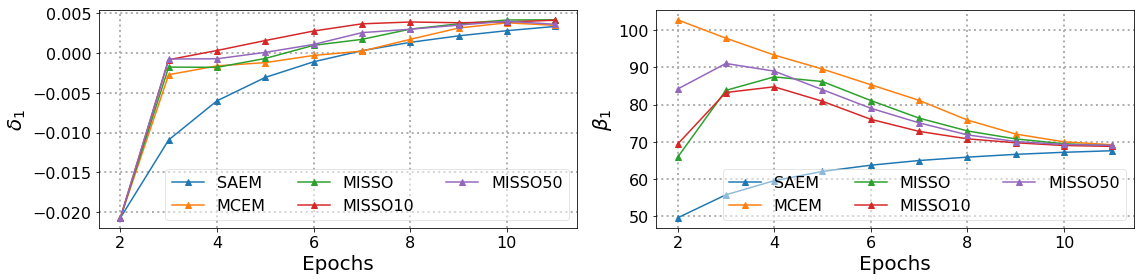
\includegraphics[width=\textwidth]{pic_paper/traumabasenoexp.png}\vspace{-.2cm}
\caption{Convergence of first component of the vector of parameters ${\bm \delta}$ and ${\bm \beta}$ for the SAEM, the MCEM and the MISSO methods. The convergence is plotted against No. of passes over the data.}\vspace{-.2cm}
\label{fig:misso_trauma}
\end{figure}

We compare in Figure~\ref{fig:misso_trauma} the convergence behavior of the estimated parameters $\bm{\beta}$ using SAEM \citep{delyon1999} (with stepsize $\gamma_k = 1/k$), MCEM \citep{wei1990mcem}  and the proposed MISSO method.
For the MISSO method, we set the batch size to $\Bsize{k} = 10 + k^2$ and we examine with selecting different number of functions in Line~\ref{line:unif} in the method -- the default settings with 1 function (MISSO), $10\%$ (MISSO10) and $50\%$ (MISSO50) of the functions per iteration.
From Figure~\ref{fig:misso_trauma}, the MISSO method converges to a static value with less number of epochs than the MCEM, SAEM methods.
It is worth noting that the difference among the MISSO runs for different number of selected functions demonstrates a variance-cost tradeoff.

\vspace{-0.05in}
\subsection{Training Bayesian CNN using MISSO}
\vspace{-0.05in}

This application follows \textbf{Example 2} described in Section~\ref{sec:framework}. We use variational inference and the ELBO loss \eqref{eq:variationalobjective} to fit Bayesian Neural Networks on different datasets.
At iteration $k$, minimizing the sum of stochastic surrogates defined as in \eqref{eq:ssur} and \eqref{pairvi} yields the following MISSO update --- {\sf step (i)} pick a function index $i_k$ uniformly on $\inter[n]$; {\sf step (ii)} sample a Monte Carlo batch $ \{ z_{m}^{(k)} \}_{m=1}^{\Bsize{k}}$ from ${\cal N}(0,\Id)$; and {\sf step (iii)}  update the parameters as
%\beq\label{eq:missoupdate}
%\hp{k} = \frac{1}{n}\sum_{i=1}^{n}{\hp{\tau_{i}^{k}}} - \frac{1}{2 \gamma} \sum_{i=1}^{n}{\hat{{\bm{m}}}^k_i}
%\eeq
\beq\label{eq:missoupdate}
\begin{split}
\mu_\ell^{(k)} = \frac{1}{n}\sum_{i=1}^{n}{\mu_\ell^{(\tau_{i}^{k})}} -  \frac{\gamma}{n}\sum_{i=1}^{n}{\hat{{\bm{\delta}}}^{(k)}_{\mu_\ell,i} } \quad \textrm{and} \quad \sigma^{(k)} = \frac{1}{n}\sum_{i=1}^{n}{\sigma^{(\tau_{i}^{k})}} - \frac{\gamma}{n} \sum_{i=1}^{n}{\hat{{\bm{\delta}}}^{(k)}_{\sigma,i} } \eqsp,
\end{split}
\eeq
where $\hat{{\bm{\delta}}}^{(k)}_{\mu_\ell,i} = \hat{{\bm{\delta}}}^{(k-1)}_{\mu_\ell,i}$ and $\hat{{\bm{\delta}}}^{(k)}_{\sigma,i} = \hat{{\bm{\delta}}}^{(k-1)}_{\sigma,i}$ for $i \neq i_k$ and:
\begin{align*}
& \hat{{\bm{\delta}}}^{(k)}_{\mu_\ell,i_k} =
  - \frac{1}{\Bsize{k}}\sum_{m=1}^{\Bsize{k}} \nabla_{w} \log p(y_{i_k} | x_{i_k}, w) \Big|_{w = t(\hp{k-1},z_m^{(k)})}  + \nabla_{\mu_\ell}  d(\hp{k-1}) \eqsp,\\
  & \hat{{\bm{\delta}}}^{(k)}_{\sigma,i_k} =
 - \frac{1}{\Bsize{k}}\sum_{m=1}^{\Bsize{k}} z_m^{(k)} \nabla_{w} \log p(y_{i_k} | x_{i_k}, w) \Big|_{w = t(\hp{k-1},z_m^{(k)})}  + \nabla_{\sigma}  d(\hp{k-1})
\end{align*}
with $d(\param) = n^{-1} \sum_{\ell=1}^{d} \left(- \log(\sigma) + (\sigma^2 + \mu_\ell^2)/2 -1/2 \right)$.

\textbf{Bayesian LeNet-5 on MNIST \citep{lecun1998gradient}:}
We apply the MISSO method to fit a Bayesian variant of LeNet-5 \citep{lecun1998gradient} (see Appendix~\ref{appendix:bnn}).
We train this network on the MNIST dataset \citep{lecun1998mnist}. The training set is composed of $n=55\,000$ handwritten digits, $28 \times 28$ images. Each image is labelled with its corresponding number (from zero to nine).
Under the prior distribution $\prior$, see \eqref{eq:vi}, the weights are assumed  independent and identically distributed according to ${\cal N}(0,1)$.
We also assume that $q(\cdot; \param) \equiv  \mathcal{N}(\mu,\sigma^2 \Id )$.
The variational posterior parameters are thus $\param = (\mu, \sigma) $ where $\mu = (\mu_\ell, \ell \in \inter[d])$ where $d$ is the number of weights in the neural network. We use the re-parametrization as $w = t(\param, z)= \mu+ \sigma  z$ with $z \sim \mathcal{N}(0, \Id)$.

We describe in Table~\ref{table:lenet} the architecture of the Convolutional Neural Network introduced in \citep{lecun1998gradient} and trained on MNIST:
\begin{table}[H]
\begin{center}
\begin{tabular}{ l c c c c r}
  \hline
  layer type & width & stride& padding & input shape& nonlinearity \\
  \hline
convolution ($5 \times 5$) & 6 & 1 & 0 & $1 \times 32 \times 32$ & ReLU \\
max-pooling ($2 \times 2$) &  & 2 & 0 & $6 \times 28 \times 28$ & \\
convolution ($5 \times 5$) & 6 & 1 & 0 & $1 \times 14 \times 14$ & ReLU \\
max-pooling ($2 \times 2$) &  & 2 & 0 & $16 \times 10 \times 10$ & \\
fully-connected & 120 &  &  & $400$ & ReLU \\
fully-connected & 84 &  &  & $ 120$ & ReLU \\
fully-connected & 10 &  &  & $ 84$ &  \\
  \hline
\end{tabular}
    \caption{LeNet-5 architecture}    \label{table:lenet}
\end{center}
\end{table}

\textbf{Bayesian ResNet-18 \citep{he2016deep} on CIFAR-10 \citep{krizhevsky2012imagenet}:}

We train here the Bayesian variant of the ResNet-18 neural network (see Appendix~\ref{appendix:resnet}) introduced in \citep{he2016deep} on CIFAR-10. 
The latter dataset is composed of $n=60\,000$ handwritten digits, $32 \times 32$ colour images in $10$ classes, with $6\,000$ images per class.
As in the previous example, the weights are assumed  independent and identically distributed according to ${\cal N}(0,1)$.
The source code used as a backbone here can be found in the TensorFlow Probability Github repo (\url{https://github.com/tensorflow/probability/blob/master/tensorflow_probability/examples/cifar10_bnn.py}) where the default hyperparameters, as the L annealing constant or the number of MC samples, were used for the benchmark methods. For better efficiency and lower variance, the Flipout estimator \citep{wen2018flipout} is preferred than a simple reparametrization trick for ResNet-18.

We describe in Table~\ref{table:resnet} the architecture of the Resnet-18 we train on CIFAR-10:
\begin{table}[H]
\begin{center}
\begin{tabular}{ l c c c c r}
  \hline
  layer type & Output Size & ResNet-18&  nonlinearity \\
  \hline
\textrm{conv1} & $112 \times 112 \times 64$ & $7 \times 7$, $64$, stride 2 & ReLU \\
\textrm{conv2x} & $ 56 \times 56 \times 64$ &$ \begin{pmatrix}
   3 \times 3, 64 \\
   3 \times 3, 64
\end{pmatrix} \times 2$& ReLU \\
\textrm{conv3x} & $ 28 \times 28 \times 128 $& $ \begin{pmatrix}
   3 \times 3, 128 \\
   3 \times 3, 128
\end{pmatrix} \times 2$ & ReLU \\
\textrm{conv4x} & $ 14 \times 14 \times 256$ &$ \begin{pmatrix}
   3 \times 3, 256 \\
   3 \times 3, 256
\end{pmatrix} \times 2$& ReLU \\
\textrm{conv5x} & $ 7 \times 7 \times 512$ &$ \begin{pmatrix}
   3 \times 3, 512 \\
   3 \times 3, 512
\end{pmatrix} \times 2$& ReLU \\
\textrm{average pool} & $ 1 \times 1 \times 512$ & $7 \times 7$ average pool & ReLU \\
\textrm{fully connected} & $1000$ & $512 \times 1000$ fully connections &  \\
\textrm{softmax} & $1000$ &  & \\
  \hline
\end{tabular}
    \caption{ResNet-18 architecture} \label{table:resnet}
\end{center}
\end{table}


\textbf{Experiment Results:}
We compare the convergence of the \textit{Monte Carlo variants} of the following state of the art optimization algorithms --- the ADAM \citep{kingma:adam}, the Momentum \citep{sutskever2013importance} and the SAG \citep{schmidt2017minimizing} methods versus the \textit{Bayes by Backprop} (BBB) \citep{blundell2015weight} and our proposed MISSO method.
For all these methods, the loss function \eqref{eq:variationalobjective} and its gradients were computed by Monte Carlo integration using Tensorflow Probability library \citep{dillon2017tfp}, based on the re-parametrization described above.
Update rules for each algorithm are performed using their vanilla implementations on TensorFlow \citep{tensorflow2015-whitepaper} as detailed in Appendix~\ref{bnn:updates}.
We use the following hyperparameters for all runs --- the learning rate is $10^{-3}$, we run $100$ epochs with a mini-batch size of $128$ and use the batchsize of $\Bsize{k} = k$.\vspace{-.2cm}


\begin{figure}[H]
    \centering
    \subfloat[LeNet-5 on MNIST]{{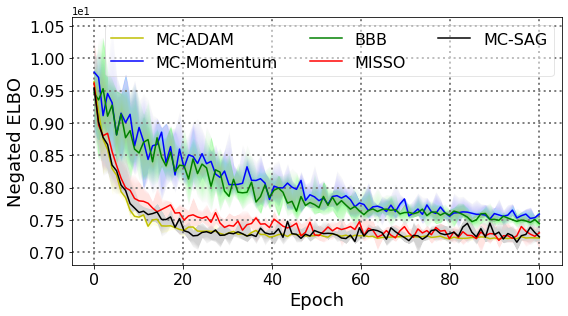
\includegraphics[width=6cm]{pic_paper/small_lenet.png} }}%
    \qquad
    \subfloat[ResNet-18 on CIFAR-10]{{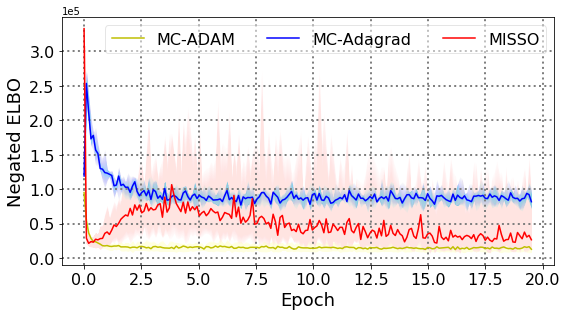
\includegraphics[width=6cm]{pic_paper/small_resnet.png} }}%
  \caption{(a)  Negated ELBO versus epochs elapsed for fitting the Bayesian LeNet-5 on MNIST using different algorithms.
(b)  ELBO versus epochs elapsed for fitting the Bayesian ResNet-18 on CIFAR-10 using different algorithms.
The solid curve is obtained from averaging over 5 independent runs of the methods, and the shaded area represents the standard deviation.}\label{fig:lenetopt}
\end{figure}



Figure~\ref{fig:lenetopt}(a) shows the convergence of the negated evidence lower bound against the number of passes over data (one pass represents an epoch). As observed, the proposed MISSO method outperforms \textit{Bayes by Backprop} and Momentum, while similar convergence rates are observed with the MISSO, ADAM and SAG methods for our experiment on MNIST dataset using a Bayesian variant of LeNet-5. 
On the other hand, the experiment conducted on CIFAR-10 (Figure~\ref{fig:lenetopt}(b)) using a much larger network, \ie\ a Bayesian variant of ResNet-18 (see Table~\ref{table:resnet}) showcases the need of a well-tuned adaptive methods to reach better training loss (and also faster). Our MISSO method is similar to the Monte Carlo variant of ADAM but slower than built-in TF optimizer Adagrad. Recall that the purpose of this paper is to provide a common class of optimizers, such as VI, in order to study their convergence behaviors, and not to introduce a novel method outperforming the baselines methods.
Figure~\ref{fig:lenetopt}(b) also highlights high variance of the MISSO estimator which would then benefit from variance reduction methods, being for now just an incremental one. We leave that research direction open for the sake of clarity of our paper.

\vspace{-0.05in}
\section{Conclusion}
\vspace{-0.05in}

We present a unifying framework for minimizing a non-convex finite-sum objective function using incremental surrogates when the latter functions are expressed as an expectation and are intractable.
Our approach covers a large class of non-convex applications in machine learning such as logistic regression with missing values and variational inference.
We provide both finite-time and asymptotic guarantees of our incremental stochastic surrogate optimization technique and illustrate our findings training a binary logistic regression with missing covariates to predict hemorrhagic shock and a Bayesian variant of LeNet-5 on MNIST.

\newpage

\bibliographystyle{abbrvnat}
\bibliography{ref}

\newpage

\appendix

\section{Proof of Theorem~\ref{thm:main}}
\begin{Theorem*}
Under S\ref{ass:sur}, S\ref{ass:diff}, H\ref{ass:sur}, H\ref{controlapprox}. For any $K_{\sf max} \in \NN$, let $K$ be an independent discrete r.v.~drawn uniformly from $\{0,...,K_{\sf max}-1\}$ and define the following quantity:
\beq \notag
\Delta_{( K_{\sf max} )} \eqdef 2 n L \EE[  \sumSur{0}{\hp{0}} - \sumSur{K_{\sf max}}{\hp{K_{\sf max}}} ] +  \sum_{k=0}^{K_{\sf max}-1} \frac{4 L C_{\sf r} }{\sqrt{\Bsize{k}}} \eqsp,
\eeq
Then we have following non-asymptotic bounds:
\beq \notag
\EE \big[ \| \grd \eSur{K}{\hp{K}} \|^2 \big] \leq \frac{\Delta_{( K_{\sf max} )}}{K_{\sf max}},~~
\EE[ g_-( \hp{K} ) ] \leq \sqrt{\frac{ \Delta_{( K_{\sf max} )} }{ K_{\sf max} }} + \frac{C_{\sf gr}}{K_{\sf max}} \sum_{k=0}^{K_{\sf max}-1} \Bsize{k}^{-1/2}.
\eeq
\end{Theorem*}
\begin{proof}
We begin by recalling the  definition
\beq
\sumSur{k}{\param} \eqdef \frac{1}{n} \sum_{i=1}^n \tafct{i}{k}{\param}.
\eeq
Notice that 
\beq
\begin{split}
\sumSur{k+1}{\param} & = \frac{1}{n} \sum_{i=1}^n \ssur{i}{\param}{\hp{\tau_i^{k+1}}}{ \{ z_{i,m}^{(\tau_i^{k+1})} \}_{m=1}^{\Bsize{\tau_i^{k+1}}} } \\
& =
\sumSur{k}{\param} + \frac{1}{n} \big( \ssur{i_k}{\param}{\hp{k}}{ \{ z_{i_k,m}^{(k)} \}_{m=1}^{\Bsize{k}}} - \ssur{i_k}{\param}{\hp{\tau_{i_k}^k}}{ \{ z_{i_k,m}^{(\tau_{i_k}^k)} \}_{m=1}^{\Bsize{\tau_{i_k}^k}}} \big).
\end{split}
\eeq
Furthermore, we recall that
\beq
\Sur{k}{\param} \eqdef {\textstyle \frac{1}{n} \sum_{i=1}^n} \sur{i}{\param}{\hp{\tau_i^k}},~~~~
\eSur{k}{\param} \eqdef \Sur{k}{\param}- {\cal L} ( \param ).
\eeq
Due to S\ref{ass:diff}, we have
\beq \label{eq:surbd}
 \| \grd \eSur{k}{\hp{k}} \|^2 \leq 2L \eSur{k}{\hp{k}}.
\eeq

%Due to S\ref{ass:sur}, $\eSur{k}{\param}$ is an $L$-smooth function, and thus the following upper bound holds with $\param_0 = \hp{k} - \frac{1}{L} \grd \eSur{k}{\hp{k}}$,
%\beq
%\eSur{k}{\param_0} \leq \eSur{k}{\hp{k}} - \frac{1}{2L} \| \grd \eSur{k}{\hp{k}} \|^2
%\eeq
%Subsequently, shuffling terms leads to
%\beq \label{eq:surbd}
% \| \grd \eSur{k}{\hp{k}} \|^2 \leq 2L (\eSur{k}{\hp{k}} - {\eSur{k}{\param_0}}) \leq 2L \eSur{k}{\hp{k}},
%\eeq
%where in the last inequality we have used ${\eSur{k}{\param_0}} \geq 0$.

To prove the first bound in \eqref{eq:misso_rate}, using the optimality of $\hp{k+1}$, one has
\beq \label{eq:firsteq}
\begin{split}
& \sumSur{k+1}{\hp{k+1}} \leq \sumSur{k+1}{\hp{k}} \\
& = \sumSur{k}{\hp{k}} + {\textstyle \frac{1}{n}} \big(
\ssur{i_k}{\hp{k}}{\hp{k}}{ \{ z_{i_k,m}^{(k)} \}_{m=1}^{\Bsize{k}} }
- \ssur{i_k}{\hp{k}}{\hp{\tau_{i_k}^k}}{ \{ z_{i_k,m}^{(\tau_{i_k}^k)} \}_{m=1}^{\Bsize{\tau_{i_k}^k}} } \big)
\end{split}
\eeq
Let ${\cal F}_k$ be the filtration of random variables up to iteration $k$, \ie $\{i_{\ell-1},\{ z_{i_{\ell-1},m}^{(\ell-1)} \}_{m=1}^{\Bsize{\ell-1}} ,\hp{\ell}\}_{\ell=1}^k$. We observe that the conditional expectation evaluates to
\beq
\begin{split}
& \EE_{i_k} \big[ \EE\big[ \ssur{i_k}{\hp{k}}{\hp{k}}{ \{ z_{i_k,m}^{(k)} \}_{m=1}^{\Bsize{k}} } | {\cal F}_k , i_k \big] | {\cal F}_k \big] \\
& = {\cal L} ( \hp{k} ) + \EE_{i_k} \big[ \EE\big[ \frac{1}{\Bsize{k}}\sum_{m=1}^{\Bsize{k}} \rsur{i_k}{\hp{k}}{\hp{k}}{z_{i_k,m}^{(k)}} - \sur{i_k}{ \hp{k} }{ \hp{k} }  | {\cal F}_k, i_k \big] | {\cal F}_k \big]  \\
& \leq {\cal L} ( \hp{k} ) +  \frac{C_{\sf r}}{\sqrt{\Bsize{k}}},
\end{split}
\eeq
where the last inequality is due to H\ref{controlapprox}.
Moreover,
\beq
\begin{split}
& \EE \big[ \ssur{i_k}{\hp{k}}{\hp{\tau_{i_k}^k}}{ \{ z_{i_k,m}^{(\tau_{i_k}^k)} \}_{m=1}^{\Bsize{\tau_{i_k}^k}} } | {\cal F}_k \big]  = \frac{1}{n} \sum_{i=1}^n  \ssur{i}{\hp{k}}{\hp{\tau_{i}^k}}{ \{ z_{i,m}^{(\tau_{i}^k)} \}_{m=1}^{\Bsize{\tau_{i}^k}} } = \sumSur{k}{\hp{k}}.
\end{split}
\eeq
Taking the conditional expectations on both sides of \eqref{eq:firsteq} and re-arranging terms give:
\beq \label{eq:afterarrange}
\sumSur{k}{\hp{k}} - {\cal L} ( \hp{k} ) \leq n \!~ \EE \big[  \sumSur{k}{\hp{k}} - \sumSur{k+1}{\hp{k+1}} |{\cal F}_k \big] +  \frac{C_{\sf r}}{\sqrt{\Bsize{k}}}
\eeq
Proceeding from \eqref{eq:afterarrange}, we observe the following lower bound for the left hand side
\beq
\begin{split}
& \sumSur{k}{\hp{k}} - {\cal L} ( \hp{k} ) \overset{(a)}{=} \sumSur{k}{\hp{k}} - \Sur{k}{\hp{k}} + \eSur{k}{\hp{k}} \\
& \overset{(b)}{\geq} \sumSur{k}{\hp{k}} - \Sur{k}{\hp{k}} + \frac{1}{2L} \| \grd \eSur{k}{\hp{k}} \|^2 \\
& = \underbrace{\frac{1}{n} \sum_{i=1}^n \Big\{ \frac{1}{\Bsize{\tau_i^k}}\sum_{m=1}^{\Bsize{\tau_i^k}} \rsur{i}{\hp{k}}{\hp{\tau_i^k}}{z_{i,m}^{(\tau_i^k)}} -  \sur{i}{\hp{k}}{\hp{\tau_i^k}} \Big\}}_{ \eqdef - \delta^{(k)}( \hp{k} ) } + \frac{1}{2L} \| \grd \eSur{k}{\hp{k}} \|^2
\end{split}
\eeq
where (a) is due to $\eSur{k}{\hp{k}} = 0$ [cf.~S\ref{ass:sur}], (b) is due to \eqref{eq:surbd} and we have defined the summation in the last equality as $- \delta^{(k)}( \hp{k} )$.
%We further obtain
%\beq
%\sumSur{k}{\hp{k}} - {\cal L} ( \hp{k} ) \geq - \delta^{(k)}( \hp{k} ) + \frac{1}{2L} \| \grd \eSur{k}{\hp{k}} \|^2
%\eeq
Substituting the above into \eqref{eq:afterarrange} yields
\beq
\frac{ \| \grd \eSur{k}{\hp{k}} \|^2}{2L} \leq n \!~ \EE \big[  \sumSur{k}{\hp{k}} - \sumSur{k+1}{\hp{k+1}} |{\cal F}_k \big] +  \frac{C_{\sf r}}{\sqrt{\Bsize{k}}} + \delta^{(k)}( \hp{k} )
\eeq
Observe the following upper bound on the total expectations:
\beq
\begin{split}
& \EE \big[ \delta^{(k)}( \hp{k} ) \big] \leq \EE \Big[ \frac{1}{n} \sum_{i=1}^n \frac{C_{\sf r}}{ \sqrt{\Bsize{\tau_i^k}} } \Big],
%& \EE \big[  \sup_{ \param \in \Param } \big( \epsilon^{(k)}(\param) \big)^2 \big]
%\leq \EE \Big[ \frac{1}{n} \sum_{i=1}^n \frac{C_{\sf gr}}{ \sqrt{\Bsize{\tau_i^k}} } \Big]
\end{split}
\eeq
which is due to H\ref{controlapprox}.
It yields
\beq \notag
\begin{split}
\EE\big[ \| \grd \eSur{k}{\hp{k}} \|^2 \big] & \leq 2nL \!~ \EE \big[  \sumSur{k}{\hp{k}} - \sumSur{k+1}{\hp{k+1}} \big] + \frac{2 L C_{\sf r}}{\sqrt{\Bsize{k}}} + \frac{1}{n}\sum_{i=1}^n \EE \Big[ \frac{ 2 L C_{\sf r} }{ \sqrt{ \Bsize{\tau_i^k} }} \Big]
\end{split}
\eeq
Finally, for any $K_{\sf max} \in \NN$, we let $K$ be a discrete r.v.~that is uniformly drawn from $\{0,1,...,K_{\sf max} - 1\}$. Using H\ref{controlapprox} and taking total expectations lead to
\beq \label{eq:prebdd}
\begin{split}
& \EE \big[\| \grd \eSur{K}{\hp{K}} \|^2 \big] = \frac{1}{K_{\sf max}} \sum_{k=0}^{K_{\sf max}-1} \EE [ \| \grd \eSur{k}{\hp{k}} \|^2 ] \\
& \leq \frac{2n L \EE[  \sumSur{0}{\hp{0}} - \sumSur{K_{\sf max}}{\hp{K_{\sf max}}} ]}{K_{\sf max}} + \frac{2L C_{\sf r}}{K_{\sf max}} \sum_{k=0}^{K_{\sf max}-1} \EE \Big[   \frac{1}{\sqrt{\Bsize{k}}} + \frac{1}{n}\sum_{i=1}^n \frac{ 1 }{ \sqrt{ \Bsize{\tau_i^k} }} \Big]
\end{split}
\eeq
For all $i \in \inter$, the index $i$ is selected with a probability equal to $\frac{1}{n}$ when conditioned independently on the past. We observe:
\begin{equation}
\EE [ \Bsize{\tau_i^k}^{-1/2}]  = \sum_{j=1}^{k} \frac{1}{n}  \left(1-\frac{1}{n}\right)^{j-1}\Bsize{k-j}^{-1/2}
\end{equation}
Taking the sum yields:
\begin{equation} \label{eq:mkcal}
\begin{split}
& \sum_{k=0}^{K_{\sf max}-1} \EE [ \Bsize{\tau_i^k}^{-1/2} ]  = \sum_{k=0}^{K_{\sf max}-1} \sum_{j=1}^k \frac{1}{n}  \left(1-\frac{1}{n}\right)^{j-1}\Bsize{k-j}^{-1/2} = \sum_{k=0}^{K_{\sf max}-1}{\sum_{l=0}^{ k-1} \frac{1}{n} \left(1-\frac{1}{n}\right)^{k-(l+1)}  \Bsize{l}^{-1/2}} \\
& = \sum_{l=0}^{K_{\sf max}-1}
%{\left(1-\frac{1}{n}\right)^{-(l+1)}
\Bsize{l}^{-1/2} \sum_{k=l+1}^{K_{\sf max}-1} \frac{1}{n} \left(1-\frac{1}{n}\right)^{k - (l+1)}  \leq \sum_{l=0}^{K_{\sf max}-1}  {\Bsize{l}^{-1/2}}
\end{split}
\end{equation}
where the last inequality is due to upper bounding the geometric series.
Plugging this back into \eqref{eq:prebdd} yields
\beq
\begin{split}
& \EE \big[ \| \grd \eSur{K}{\hp{K}} \|^2 \big] = \frac{1}{K_{\sf max}} \sum_{k=0}^{K_{\sf max}-1} \EE [ \| \grd \eSur{k}{\hp{k}} \|^2 ] \\
& \leq \frac{2 n L \EE[  \sumSur{0}{\hp{0}} - \sumSur{K_{\sf max}}{\hp{K_{\sf max}}} ]}{K_{\sf max}} + \frac{1}{K_{\sf max}} \sum_{k=0}^{K_{\sf max}-1} \frac{4 L C_{\sf r} }{\sqrt{\Bsize{k}}} = \frac{ \Delta_{( K_{\sf max} )} }{ K_{\sf max} }.
\end{split}
\eeq
This concludes our proof for the first inequality in \eqref{eq:misso_rate}.

To prove the second inequality of \eqref{eq:misso_rate}, we define the shorthand notations $g^{(k)} \eqdef g( \hp{k} )$, $g_-^{(k)} \eqdef - \min\{0, g^{(k)} \}$, $g_+^{(k)} \eqdef \max\{0, g^{(k)} \}$.
We observe that
\beq
\begin{split}
g^{(k)} & = \inf_{ \param \in \Param } \frac{ {\cal L}'( \hp{k} , \param - \hp{k} ) }{ \| \hp{k} - \param \|} \\
& = \inf_{ \param \in \Param }  \Big\{ \frac{ \frac{1}{n} \sum_{i=1}^n \widehat{\cal L}_i^{'}( \hp{k} , \param - \hp{k} ; \hp{ \tau_i^k } ) }{ \| \hp{k} - \param \|} -
\frac{ \pscal{\grd \eSur{k}{\hp{k}} }{ \param - \hp{k} } }{{ \| \hp{k} - \param \|} } \Big\} \\
& \geq - \| \grd \eSur{k}{\hp{k}} \| + \inf_{ \param \in \Param } \frac{ \frac{1}{n} \sum_{i=1}^n \widehat{\cal L}_i^{'}( \hp{k} , \param - \hp{k} ; \hp{ \tau_i^k } ) }{ \| \hp{k} - \param \|}
\end{split}
\eeq
%\beq
%g^{(k)} \geq - \| \grd \eSur{k}{\hp{k}} \| + \sup_{ \param \in \Param } \frac{ \frac{1}{n} \sum_{i=1}^n \widehat{\cal L}_i^{'}( \hp{k} , \hp{k} - \param ; \hp{ \tau_i^k } ) }{ \| \hp{k} - \param \|}
%\eeq
where the last inequality is due to the Cauchy-Schwarz inequality and we have defined $\widehat{\cal L}_i'( \param , {\bm d}; \hp{\tau_i^k} )$ as the directional derivative of $\widehat{\cal L}_i ( \cdot ; \hp{\tau_i^k} ) $ at $\param$ along the direction ${\bm d}$. Moreover, for any $\param \in \Param$,
\beq
\begin{split}
& \frac{1}{n} \sum_{i=1}^n \widehat{\cal L}_i^{'}( \hp{k} , \param - \hp{k} ; \hp{ \tau_i^k } )\\
& = \underbrace{\widetilde{\cal L}^{(k) '} ( \hp{k}, \param - \hp{k} )}_{\geq 0} - \widetilde{\cal L}^{(k) '} ( \hp{k}, \param - \hp{k} ) +
 \frac{1}{n} \sum_{i=1}^n \widehat{\cal L}_i^{'}( \hp{k} , \param - \hp{k} ; \hp{ \tau_i^k } ) \\
& \geq
 \frac{1}{n} \sum_{i=1}^n \Big\{ \widehat{\cal L}_i^{'}( \hp{k} , \param - \hp{k} ; \hp{ \tau_i^k } ) - \frac{1}{\Bsize{\tau_i^k}} \sum_{m=1}^{\Bsize{\tau_i^k}} r_i' ( \hp{k}, \param - \hp{k}; \hp{\tau_i^k} , z_{i,m}^{(\tau_i^k)} ) \Big\}
 \end{split}
\eeq
where the inequality is due to the optimality of $\hp{k}$ and the convexity of $\sumSur{k}{\param}$ [cf.~H\ref{ass:lips}]. Denoting a scaled version of the above term as:
\beq \notag
\epsilon^{(k)} ( \param) \eqdef \frac{ \frac{1}{n} \sum_{i=1}^n \Big\{ \frac{1}{\Bsize{\tau_i^k}} \sum_{m=1}^{\Bsize{\tau_i^k}} r_i' ( \hp{k}, \param - \hp{k} ; \hp{\tau_i^k} , z_{i,m}^{(\tau_i^k)} ) - \widehat{\cal L}_i^{'}( \hp{k} , \param - \hp{k} ; \hp{ \tau_i^k } )  \Big\} }{\| \hp{k} - \param \|}.
\eeq
We have
\beq \label{eq:gksur}
g^{(k)} \geq - \| \grd \eSur{k}{\hp{k}} \| + \inf_{\param \in \Param} (-\epsilon^{(k)}(\param)) \geq
 - \| \grd \eSur{k}{\hp{k}} \| - \sup_{\param \in \Param} |\epsilon^{(k)}(\param)|.
\eeq
Since $g^{(k)} = g_+^{(k)} - g_-^{(k)}$ and $g_+^{(k)} g_-^{(k)} = 0$, this implies
\beq \label{eq:gmbd}
g_-^{(k)} \leq \| \grd \eSur{k}{\hp{k}} \| + \sup_{\param \in \Param} |\epsilon^{(k)}(\param)|.
\eeq
Consider the above inequality  when $k=K$, \ie the random index, and taking total expectations on both sides gives
\beq
\EE [ g_-^{(K)} ] \leq \EE[ \| \grd \eSur{K}{\hp{K}} \| ] + \EE[ \sup_{\param \in \Param} \epsilon^{(K)}(\param) ]
\eeq
We note that
\beq
\Big( \EE[ \| \grd \eSur{K}{\hp{K}} \| ] \Big)^2 \leq \EE[ \| \grd \eSur{K}{\hp{K}} \|^2 ] \leq \frac{ \Delta(K_{\sf max}) }{ K_{\sf max} },
\eeq
where the first inequality is due to the convexity of $(\cdot)^2$ and the Jensen's inequality,
and
\beq
\begin{split}
\EE[ \sup_{\param \in \Param} \epsilon^{(K)}(\param) ] & = \frac{1}{K_{\sf max}} \sum_{k=0}^{K_{\sf max}} \EE[ \sup_{\param \in \Param} \epsilon^{(k)}(\param) ] \overset{(a)}{\leq}
\frac{C_{\sf gr}}{K_{\sf max}} \sum_{k=0}^{K_{\sf max}-1} \EE\Big[ \frac{1}{n}\sum_{i=1}^n \Bsize{\tau_i^k}^{-1/2} \Big] \\
& \overset{(b)}{\leq}
\frac{C_{\sf gr}}{K_{\sf max}} \sum_{k=0}^{K_{\sf max}-1} \Bsize{k}^{-1/2}
\end{split}
\eeq
where (a) is due to H\ref{controlapprox} and (b) is due to \eqref{eq:mkcal}.
This implies
\beq
\EE [ g_-^{(K)} ] \leq \sqrt{ \frac{\Delta_{(K_{\sf max})}}{K_{\sf max}} } + \frac{C_{\sf gr}}{K_{\sf max}} \sum_{k=0}^{K_{\sf max}-1} \Bsize{k}^{-1/2},
\eeq
and concludes the proof of the theorem.
\end{proof}

\section{Proof of Theorem~\ref{thm:mainasymp}}
\begin{Theorem*}
Under S\ref{ass:sur}, S\ref{ass:diff}, H\ref{ass:sur}, H\ref{controlapprox}. In addition, assume that $\{\Bsize{k}\}_{k \geq 0}$ is a non-decreasing sequence of integers which satisfies $\sum_{k=0}^{\infty}{\Bsize{k}^{-1/2}} < \infty$. Then:
\begin{enumerate}[leftmargin=.75cm]
\item the negative part of the stationarity measure converges almost surely to zero, \ie $\textstyle \lim_{ k \rightarrow \infty} g_-( \hp{k}) = 0$ a.s.. 
\item the objective value ${\cal L} ( \hp{k} )$ converges almost surely to a finite number $\underline{\cal L}$, \ie $\lim_{k \rightarrow \infty} {\cal L} ( \hp{k} ) = \underline{\cal L}$ a.s..
\end{enumerate}
\end{Theorem*}
\begin{proof}
We apply the following auxiliary lemma which proof can be found in Appendix~\ref{appendix:lemma} for the readability of the current proof:
\begin{Lemma}\label{lemmars}
Let $\left(V_k \right)_{k\geq0}$ be a non negative sequence of random variables such that $\EE[V_0] < \infty$. Let $\left(X_k \right)_{k\geq0}$ a non negative sequence of random variables and $\left(E_k \right)_{k \geq 0}$ be a sequence of random variables such that $\sum_{k=0}^{\infty}{\EE[|E_k|]} < \infty$. If for any $k \geq 1$:
\begin{equation}
V_{k} \leq V_{k-1} - X_{k-1} + E_{k-1}
\end{equation}
 then:
\begin{enumerate}[label=(\roman*)]
\item for all $k \geq 0$, $\EE[V_k] < \infty$ and the sequence $\left(V_k \right)_{k\geq0}$  converges a.s. to a finite limit $V_{\infty}$.
\item the sequence $\left(\EE[V_k] \right)_{k\geq0}$ converges and $\lim \limits_{k \to \infty}\EE[V_k] = \EE[V_{\infty}] $.
\item the series $\sum_{k=0}^{\infty}{X_k}$ converges almost surely and $\sum_{k=0}^{\infty}{\EE[X_k]}< \infty$.
\end{enumerate}
\end{Lemma}
We proceed from \eqref{eq:firsteq} by re-arranging terms and observing that
\beq
\begin{split}
 \Sur{k+1}{\hp{k+1}} & \leq \Sur{k}{\hp{k}} - {\textstyle \frac{1}{n}} \big( \sur{i_k}{\hp{k}}{\hp{\tau_{i_k}^k}} - \sur{i_k}{\hp{k}}{\hp{k}} \big)  \\
& - \big( \sumSur{k+1}{\hp{k+1}} - \Sur{k+1}{\hp{k+1}} \big) + \big( \sumSur{k}{\hp{k}} - \Sur{k}{\hp{k}} \big) \\
& + {\textstyle \frac{1}{n}} \big(
\ssur{i_k}{\hp{k}}{\hp{k}}{ \{ z_{i_k,m}^{(k)} \}_{m=1}^{\Bsize{k}} } - \sur{i_k}{\hp{k}}{\hp{k}} \big) \\
& + {\textstyle \frac{1}{n}} \big( \sur{i_k}{\hp{k}}{\hp{\tau_{i_k}^k}}
- \ssur{i_k}{\hp{k}}{\hp{\tau_{i_k}^k}}{ \{ z_{i_k,m}^{(\tau_{i_k}^k)} \}_{m=1}^{\Bsize{\tau_{i_k}^k}} } \big)
\end{split}
\eeq
Our idea is to apply Lemma~\ref{lemmars}.
Under S\ref{ass:sur}, the finite sum of surrogate functions $\Sur{k}{\param}$, defined in \eqref{eq:sumsurrodet}, is lower bounded by a constant $c_k > - \infty$ for any $\param$. To this end, we observe that
\beq \label{eq:dvk}
V_k \eqdef \Sur{k}{\hp{k}} - \inf_{k \geq 0} c_k \geq 0
\eeq
is a non-negative random variable.

Secondly, under H\ref{ass:sur}, the following random variable is non-negative
\beq \label{eq:dxk}
X_{k} \eqdef {\textstyle \frac{1}{n}} \big( \sur{i_k}{\hp{\tau_{i_k}^k}}{\hp{k}} - \sur{i_k}{\hp{k}}{\hp{k}} \big) \geq 0.
\eeq

Thirdly, we define
\beq \label{eq:dek}
\begin{split}
E_{k} & = - \big( \sumSur{k+1}{\hp{k+1}} - \Sur{k+1}{\hp{k+1}} \big) + \big( \sumSur{k}{\hp{k}} - \Sur{k}{\hp{k}} \big) \\
& + {\textstyle \frac{1}{n}} \big(
\ssur{i_k}{\hp{k}}{\hp{k}}{ \{ z_{i_k,m}^{(k)} \}_{m=1}^{\Bsize{k}} } - \sur{i_k}{\hp{k}}{\hp{k}} \big) \\
& + {\textstyle \frac{1}{n}} \big( \sur{i_k}{\hp{k}}{\hp{\tau_{i_k}^k}}
- \ssur{i_k}{\hp{k}}{\hp{\tau_{i_k}^k}}{ \{ z_{i_k,m}^{(\tau_{i_k}^k)} \}_{m=1}^{\Bsize{\tau_{i_k}^k}} } \big).
\end{split}
\eeq
Note that from the definitions \eqref{eq:dvk}, \eqref{eq:dxk}, \eqref{eq:dek}, we have
$V_{k+1} \leq V_k - X_k + E_k$ for any $k \geq 1$.

Under H\ref{controlapprox}, we observe that
\beq
\EE \big[ | \ssur{i_k}{\hp{k}}{\hp{k}}{ \{ z_{i_k,m}^{(k)} \}_{m=1}^{\Bsize{k}} } - \sur{i_k}{\hp{k}}{\hp{k}} | \big] \leq C_{\sf r} \Bsize{k}^{-1/2}
\eeq
\beq
\EE \Big[ \Big| \sur{i_k}{\hp{k}}{\hp{\tau_{i_k}^k}}
- \ssur{i_k}{\hp{k}}{\hp{\tau_{i_k}^k}}{ \{ z_{i_k,m}^{(\tau_{i_k}^k)} \}_{m=1}^{\Bsize{\tau_{i_k}^k}} } \Big| \Big] \leq C_{\sf r} \EE \Big[ \Bsize{\tau_{i_k}^k}^{-1/2}  \Big]
\eeq
\beq
\EE \big[ | \sumSur{k}{\hp{k}} - \Sur{k}{\hp{k}} | \big] \leq {\textstyle \frac{1}{n} \sum_{i=1}^n}
 C_{\sf r} \EE \Big[ \Bsize{\tau_{i}^k}^{-1/2}  \Big]
\eeq
Therefore,
\beq
\EE \big[ | E_{k} | \big] \leq {\textstyle \frac{C_{\sf r}}{n}}  \Big( \Bsize{k}^{-1/2} +
\EE \Big[ \Bsize{\tau_{i_k}^k}^{-1/2} + {\textstyle \sum_{i=1}^n} \big\{ \Bsize{\tau_{i}^k}^{-1/2} + \Bsize{\tau_{i}^{k+1}}^{-1/2} \big\} \Big] \Big)
\eeq
Using \eqref{eq:mkcal} and the assumption on the sequence $\{\Bsize{k}\}_{k \geq 0}$, we obtain that
\beq
\sum_{k=0}^\infty \EE \big[ | E_{k} | \big] < {\frac{C_{\sf r}}{n}} (2 + 2n ){\sum_{k=0}^\infty} \Bsize{k}^{-1/2}  < \infty.
\eeq
Therefore, the conclusions in Lemma~\ref{lemmars} hold. Precisely, we have $\sum_{k=0}^\infty X_k < \infty$ and $\sum_{k=0}^\infty \EE[ X_k ] < \infty$ almost surely.
Note that this implies
\beq
\begin{split}
\infty & > \sum_{k=0}^\infty \EE[ X_k ] = \frac{1}{n} \sum_{k = 0}^\infty \EE \big[ \sur{i_k}{\hp{k}}{\hp{\tau_{i_k}^k}} - \sur{i_k}{\hp{k}}{\hp{k}} \big] \\
& = \frac{1}{n} \sum_{k = 0}^\infty \EE \big[ \Sur{k}{\hp{k}} - {\cal L}( \hp{k}) \big] = \frac{1}{n} \sum_{k=0}^\infty \EE\big[ \eSur{k}{\hp{k}} \big]
\end{split}
\eeq
Since $\eSur{k}{\hp{k}} \geq 0$, the above implies
\beq \label{eq:esur}
\lim_{ k \rightarrow \infty } \eSur{k}{\hp{k}} = 0~~~\text{a.s.}
\eeq
and subsequently applying \eqref{eq:surbd}, we have $\lim_{ k \rightarrow \infty } \| \eSur{k}{\hp{k}} \| = 0$ almost surely. Finally, it follows from \eqref{eq:surbd} and \eqref{eq:gmbd} that
\beq
\lim_{k \rightarrow \infty} g_-^{(k)} \leq \lim_{k \rightarrow \infty} \sqrt{2L} \sqrt{ \eSur{k}{\hp{k}} } + \lim_{k \rightarrow \infty} \sup_{\param \in \Param} |\epsilon^{(k)}(\param)| = 0,
\eeq
where the last equality holds almost surely due to the fact that $\sum_{k=0}^\infty \EE[ \sup_{\param \in \Param} |\epsilon^{(k)}(\param)| ] < \infty$.
This concludes the asymptotic convergence of the MISSO method.

Finally, we prove that ${\cal L}(\hp{k})$ converges almost surely. As a consequence of Lemma~\ref{lemmars}, it is clear that $\{ V_k \}_{k \geq 0}$ converges almost surely and so is $\{ \Sur{k}{\hp{k}} \}_{k \geq 0}$, \ie we have $\lim_{k \rightarrow \infty} \Sur{k}{\hp{k}} = \underline{\cal L}$. Applying \eqref{eq:esur} implies that
\beq
\underline{\cal L} = \lim_{ k \rightarrow \infty } \Sur{k}{\hp{k}} = \lim_{k \rightarrow \infty} {\cal L} (\hp{k})~~~~\text{a.s.}
\eeq
This shows that ${\cal L}(\hp{k})$ converges almost surely to $\underline{\cal L}$.
\end{proof}

 \section{Proof of Lemma~\ref{lemmars}}\label{appendix:lemma}
\begin{Lemma*}
Let $\left(V_k \right)_{k\geq0}$ be a non negative sequence of random variables such that $\EE[V_0] < \infty$. Let $\left(X_k \right)_{k\geq0}$ a non negative sequence of random variables and $\left(E_k \right)_{k \geq 0}$ be a sequence of random variables such that $\sum_{k=0}^{\infty}{\EE[|E_k|]} < \infty$. If for any $k \geq 1$:
\begin{equation}\notag
V_{k} \leq V_{k-1} - X_{k-1} + E_{k-1}
\end{equation}
 then:
\begin{enumerate}[label=(\roman*)]
\item for all $k \geq 0$, $\EE[V_k] < \infty$ and the sequence $\left(V_k \right)_{k\geq0}$  converges a.s. to a finite limit $V_{\infty}$.
\item the sequence $\left(\EE[V_k] \right)_{k\geq0}$ converges and $\lim \limits_{k \to \infty}\EE[V_k] = \EE[V_{\infty}] $.
\item the series $\sum_{k=0}^{\infty}{X_k}$ converges almost surely and $\sum_{k=0}^{\infty}{\EE[X_k]}< \infty$.
\end{enumerate}
\end{Lemma*}
\begin{proof}
  We first show that for all $k \geq 0$, $\EE[V_k] < \infty$. Note indeed that:
\begin{equation}
0 \leq V_k \leq V_0 - \sum_{j=1}^{k}{X_j} + \sum_{j=1}^{k}{E_j}\leq V_0 + \sum_{j=1}^{k}{E_j}
\end{equation}
showing that $\EE[V_k] \leq \EE[V_0] + \EE\left[\sum_{j=1}^{k}{E_j}\right] < \infty$.

Since $0 \leq X_k \leq V_{k-1} - V_k + E_k$ we also obtain for all $k \geq 0$, $\EE[X_k] < \infty$. Moreover, since $\EE\left[\sum_{j=1}^{\infty}{|E_j|}\right] < \infty$, the series $\sum_{j=1}^{\infty}{E_j}$ converges a.s. We may therefore define:
\begin{equation}
W_k = V_k + \sum_{j=k+1}^{\infty}{E_j}
\end{equation}
Note that $\EE[|W_k|] \leq \EE[V_k]+\EE\left[\sum_{j=k+1}^{\infty}{|E_j|}\right] < \infty $. For all $k \geq 1$, we get:
\begin{equation}\label{chik}
\begin{split}
& W_{k} \leq V_{k-1} - X_{k} + \sum_{j=k}^{\infty}{E_j} \leq W_{k-1} - X_{k}\leq W_{k-1}\\
&\EE[W_k] \leq \EE[W_{k-1}] - \EE[X_{k}]
\end{split}
\end{equation}
Hence the sequences $(W_k)_{k\geq0}$ and $\left(\EE[W_k] \right)_{k\geq0}$ are non increasing. Since for all $k \geq 0$, $W_k \geq -  \sum_{j=1}^{\infty}{|E_j|} > -\infty$ and $\EE[W_k] \geq -  \sum_{j=1}^{\infty}{\EE[|E_j|]} > -\infty$, the (random) sequence $(W_k)_{k\geq0}$ converges a.s. to a limit $W_{\infty}$ and the (deterministic) sequence $\left(\EE[W_k] \right)_{k\geq0}$ converges to a limit $w_{\infty}$. Since $|W_k| \leq V_0 +  \sum_{j=1}^{\infty}{|E_j|}$, the Fatou lemma implies that:
\begin{equation}
\EE[\liminf \limits_{k \to \infty} |W_k|] = \EE[|W_{\infty}|] \leq \liminf \limits_{k \to \infty} \EE[|W_{k}|] \leq \EE[V_{0}] + \sum_{j=1}^{\infty}{\EE[|E_j|]}< \infty
\end{equation}
showing that the random variable $W_{\infty}$  is integrable.

In the sequel, set $U_k \triangleq W_0 - W_k$. By construction we have for all $k \geq 0$, $U_k \geq 0$, $U_k \leq U_{k+1}$ and $\EE[U_k] \leq \EE[|W_0|] + \EE[|W_k|] < \infty$ and by the monotone convergence theorem, we get:
\begin{equation}
    \lim \limits_{k \to \infty} \EE[U_k] = \EE[\lim \limits_{k \to \infty}U_k]
\end{equation}
Finally, we have:
\begin{equation}
\lim \limits_{k \to \infty} \EE[U_k] = \EE[W_0] - w_{\infty} \quad \textrm{and} \quad \EE[\lim \limits_{k \to \infty}U_k] = \EE[W_0] - \EE[W_{\infty}]
\end{equation}
showing that $\EE[W_{\infty}] = w_{\infty}$ and concluding the proof of (ii). Moreover, using \eqref{chik} we have that $W_k \leq W_{k-1} - X_k$ which yields:
\begin{equation}
\begin{split}
    & \sum_{j=1}^{\infty}{X_j} \leq W_{0} - W_{\infty} < \infty\\
    & \sum_{j=1}^{\infty}{\EE[X_j]} \leq \EE[W_{0}] - w_{\infty} < \infty
\end{split}
\end{equation}
which concludes the proof of the lemma.
\end{proof}

\clearpage

 \section{Details about the Numerical Experiments}
 
 \subsection{Binary Logistic Regression on the Traumabase}
 
 
  \subsubsection{Traumabase quantitative variables}\label{appendix:variables}
  The list of the 16 quantitative variables we use in our experiments are as follows --- \textit{age, weight, height, BMI (Body Mass Index), the Glasgow Coma Scale, the Glasgow Coma Scale motor component, the minimum systolic blood pressure, the minimum diastolic blood pressure, the maximum number of heart rate (or pulse) per unit time (usually a minute), the systolic blood pressure at arrival of ambulance, the diastolic blood pressure at arrival of ambulance, the heart rate at arrival of ambulance, the capillary Hemoglobin concentration, the oxygen saturation, the fluid expansion colloids, the fluid expansion cristalloids, the pulse pressure for the minimum value of diastolic and systolic blood pressure, the pulse pressure at arrival of ambulance.}


% \subsubsection{MISSO, MCEM and SAEM for Curved Exponential Family}\label{curvedexpo}
%Consider the case where the complete model $\param \to f_i(z_i,\param)$ belongs to the curved exponential family. For all $i \in \inter$ and $\param \in \Param$, one has:
%\begin{equation} \label{eq:complete_log}
%\log f_i(z_i,\param) = H_i(z_i) -\psi_i(\param) + \pscal{ \tilde{S}_i(z_i)} { \phi_i(\param)}.
%\end{equation}
%where $\psi_i: \param \mapsto \mathbb{R}$ and $\phi_i: \param \mapsto \mathbb{R}$ are twice continuously differentiable functions of $\param$, $H_i: \Zset \mapsto \mathbb{R}$ is a twice continuously differentiable function of $z_i$ and $\tilde{S}_i: \Zset \mapsto \mathsf{S}_i$ is a statistic taking its values in a convex subset $\mathsf{S}_i$ of $\mathbb{R}$ and such that $\int_{\Zset}{|\tilde{S}_i(z_i)|p_i(z_i,\param) \mu_i(\dz_i)} < \infty$.
%Finally, the $i$th loss function is given by
%\beq
%{\cal L}_i( \param ) = - \log \int_{\Zset} f_i(z_i,\param) \mu_i( \dz_i).
%\eeq
%
%To derive the surrogate function for this example, we follow from \textbf{Example 1} in Section~\ref{sec:framework} by taking $p(z_i , \op) = f( z_i , \op ) / g (\op)$ to yield
%\beq
%{\cal L}_i( \param ) \leq \sur{i}{\param}{\op} \eqdef \text{constant} + \int_{\Zset} \big\{ -\log f_i( z_i , \param) \} p(z_i,\op) \mu_i( \dz_i)
%\eeq
%Using \eqref{eq:complete_log}, the latter integral can be further expressed as
%\beq \label{eq:surrogate_em}
%\text{constant}  + \psi_i( \param ) - \int_{\Zset} \pscal{ \tilde{S}_i(z_i)} { \phi_i(\param)} p(z_i,\op) \mu_i( \dz_i).
%\eeq
%To summarize, we observe that the surrogate function can be written as
%$\sur{i}{\param}{\op} = \text{constant}  + \psi_i( \param ) - \pscal{ \int_{\Zset} \tilde{S}_i(z_i) p(z_i,\op) \mu_i( \dz_i) } { \phi_i(\param)}$. As suggested in the MISSO method, we note that the integral can be approximated using sample averages.
%
%Now consider the following function $L(s; \param)$:
%\begin{equation}\label{curvedL}
%L(s;\param) \eqdef \frac{1}{n} \sum_{i=1}^n \Big\{ {\psi_i(\param)} - \pscal{ s_i}{ \phi_i(\param)} \Big\},
%\end{equation}
% for all $\param \in \Param$ and $s = (s_i, 1 \leq i \leq N) \in \mathsf{S} \eqdef \times_{n=1}^N \mathsf{S}_i$.
%As noted from \eqref{eq:surrogate_em}, when $s_i$ is obtained from an appropriately sampling procedure, \eqref{curvedL} constitutes the summed stochastic surrogate function $\widetilde{\cal L}(\param)$ as suggested in the MISSO method [cf.~\Cref{alg:misso}].
%For simplicity, we consider a case when the minimization \wrt $\param$ can be uniquely attained and we denote $\hp{ s } \eqdef \argmin_{\param \in \Param} L( s; \param )$.
%We note that for this special case, the MISSO method can be compactly described in \Cref{alg:mbmcem-expo}.
%
%        \begin{algorithm}[t]
%        \algsetup{indent=1em}
%        \begin{algorithmic}[1]
%\STATE \textbf{Initialization}: given an initial parameter estimate $\hp{0}$, for all $i \in \inter$, sample a Monte Carlo batch $\{z_{i,m}^{(0)}\}_{m=1}^{\Bsize{0}}$ from  $p(z_i,\hp{0})$ and compute $s^{(0)}_{i} = \frac{1}{\Bsize{0}}\sum_{m=1}^{\Bsize{0}}{\tilde{S}_i(z^{(0)}_{i,m})}$.
%\FOR{$k=0,1...,$}
%\STATE Pick a function index $i_k$ uniformly on $\inter$. \label{line:mcem1}
%\STATE Draw $\Bsize{k}$ Monte-Carlo samples $\{z^{(k)}_{i,m}\}_{m=1}^{\Bsize{k}}$ from  $p(z_i,\hp{k-1})$.
%\STATE Update the individual sufficient statistics recursively --- for each $i \in \inter$,
%\beq \label{eq:missoem}
%s_i^{(k)} =
%  \begin{cases}
%  \frac{1}{\Bsize{k}}\sum_{m=1}^{\Bsize{k}}{\tilde{S}_i(z^{(k)}_{i,m})}        & \text{if } i = i_k \\
%  s_i^{(k-1)}                                        & \text{otherwise}
%  \end{cases}
%\eeq \label{line:mcem3}
%\STATE Set $\hp{k} = \hat{\param} \big( s^{(k)} \big) = \argmin_{ \param \in \Param } L( s^{(k)} ; \param )$ where $ s^{(k)} = (s_i^{(k)}, 1 \leq i \leq n)$.
%\ENDFOR
%\end{algorithmic}
%\caption{MISSO for curved exponential family} \label{alg:mbmcem-expo}
%        \end{algorithm}
%
%Now, in the context of the logistic regression described in section \ref{logisticreg}, for all $i \in \inter$, the complete log likelihood is expressed as:
%\beq \notag
%\log f_i(z_i,\param) \propto -y_i \delta^\top \bar{z}_i - \log \big( 1 +  \exp(- \delta^\top \bar{z}_i) \big) - \frac{1}{2}\log(|{\bm \Omega}|) + \frac{1}{2}{\rm Tr} \left({\bm \Omega}^{-1}(z_i - {\bm \beta})(z_i - {\bm \beta})^\top \right)  .
%\eeq
%For all $i \in \inter$, the sufficient statistics is $\tilde{S}_i(z_i) \triangleq ( z_i, z_iz_i^\top) $ and the minimizing map $s \to \hat{\param}(s)$ can be derived as:
%\begin{align}
%%\hat{\param}:& \mathsf{S} \mapsto \Theta \nonumber \\
%& \hat{\param} \big( (s_{i,1}, s_{i,2})_{i=1}^{n} \big) = \left(\frac{1}{n}\sum_{i=1}^{n}{s_{i,1}},\frac{1}{n}\sum_{i=1}^{n}{s_{i,2}} - \frac{1}{n^2}\sum_{i=1}^{n}{s_{i,1}} \Big(\sum_{i=1}^{n}{s_{i,1}} \Big)^\top\right)
%\end{align}
%
%Let us compare the MISSO method to the MCEM, SAEM methods as follows.
%First we note that the MISSO method differs from the MCEM method in that the latter picks \emph{all the data sample} at each iteration, \ie Line~\ref{line:mcem1} to \ref{line:mcem3} is performed for every $i \in \inter$ instead of only one randomly chosen $i_k \in \inter$. Second, the SAEM method consists of a different update of the individual sufficient statistics --- at iteration $k$ and for all $i \in \inter$, the SAEM updates the quantity $s_i^{(k)}$ as follows:
%\beq
%s_i^{(k)} = s_i^{(k-1)} + \gamma_k \left (\frac{1}{\Bsize{k}}\sum_{m=1}^{\Bsize{k}}{\tilde{S}_i(z^{(k)}_{i,m})}  - s_i^{(k-1)} \right)
%\eeq
%where $\{\gamma_k \}_{k > 0}$ is a decreasing sequence of stepsizes. Note that when $\gamma_k = 1$, the above update recovers the MCEM method.

\subsubsection{Metropolis Hastings algorithm}\label{app:trauma_mh}
During the simulation step of the MISSO method, the sampling from the target distribution $\pi(z_{i,\mis}; \param) \eqdef p(z_{i,\mis}|z_{i,\obs}, y_i;\param)$ is performed using a Metropolis Hastings (MH) algorithm \citep{meyn2012markov} with proposal distribution $q(z_{i,\mis}; {\bm \delta}) \eqdef p(z_{i,\mis}|z_{i,\obs};{\bm \delta})$ where $\param = (\beta, \Omega)$ and ${\bm \delta} = (\xi, \Sigma)$. The parameters of the Gaussian conditional distribution of $z_{i,\mis}|z_{i,\obs}$ read:
\beq
\begin{split}
&\xi = \beta_{miss} + \Omega_{mis, obs}\Omega_{obs, obs}^{-1} (z_{i,\obs} - \beta_{obs}) \eqsp,\\
&\Sigma = \Omega_{mis, mis}+ \Omega_{mis, obs}\Omega_{obs, obs}^{-1} \Omega_{obs,\mis}
\end{split}
\eeq
where we have used the Schur Complement of $\Omega_{obs, obs}$ in $\Omega$ and noted $\beta_{mis}$ (resp. $\beta_{obs}$) the missing (resp. observed) elements of $\beta$.
The MH algorithm is summarized in \Cref{alg:mh}.
\begin{algorithm}[H]
\algsetup{indent=1em}
\begin{algorithmic}[1]
\STATE \textbf{Input:} initialization $z_{i,\mis,0} \sim q(z_{i,\mis}; {\bm \delta})$
\FOR {$m=1, \cdots ,M$}
\STATE Sample $z_{i,\mis,m} \sim q(z_{i,\mis}; {\bm \delta})$
\STATE Sample $u \sim \mathcal{U}(\llbracket 0, 1 \rrbracket)$
\STATE Calculate the ratio $r = \frac{\pi(z_{i,\mis,m}; \param)/q(z_{i,\mis,m}); {\bm \delta})}{\pi(z_{i,\mis,m-1}; \param)/q(z_{i,\mis,m-1}); {\bm \delta})}$
\IF{$u < r$}
\STATE Accept $z_{i,\mis,m}$
\ELSE
\STATE $z_{i,\mis,m} \leftarrow z_{i,\mis,m-1}$
\ENDIF
\ENDFOR
\STATE \textbf{Output:} $z_{i,\mis,M}$
\end{algorithmic}
\caption{MH aglorithm}
\label{alg:mh}
        \end{algorithm}

\subsubsection{MISSO Update}\label{app:update_logistic}

\textbf{Choice of surrogate function for MISO:}
We recall the MISO deterministic surrogate defined in \eqref{pairmcem}:
\beq
\sur{i}{\param}{\op} = \int_{\Zset} \log \left(p_i(z_{i,\mis},\op)/f_i(z_{i,\mis},\param)\right) \!~ p_i( z_{i,\mis}, \op ) \mu_i ( \dz_i ) \eqsp.
\eeq
where $\param = (\delta, \beta, \Omega)$ and $\op = (\bar{\delta}, \bar{\beta}, \bar{\Omega})$.
We adapt it to our missing covariates problem and decompose the the surrogate function defined above into an observed and a missing part.

\textbf{Surrogate function decomposition}
We adapt it to our missing covariates problem and decompose the term depending on $\theta$, while $\bar{\theta}$ is fixed, in two following parts leading to
\beq \label{eq:surrogatedet}
\begin{split}
\sur{i}{\param}{\op} &= - \int_{\Zset} \log f_i(z_{i,\mis},z_{i,\obs},\param) \!~ p_i( z_{i,\mis}, \op ) \mu_i ( \dz_{i,\mis} )\\
&= - \int_{\Zset} \log \left[ p_i(y_i|z_{i,\mis},z_{i,\obs},\delta) p_i(z_{i,\mis},\beta, \Omega)\right] \!~ p_i( z_i, \op ) \mu_i (\dz_{i,\mis})\\
&= \underbrace{ - \int_{\Zset} \log p_i(y_i|z_{i,\mis},z_{i,\obs},\delta) \!~ p_i( z_i, \op ) \mu_i ( \dz_{i,\mis} )}_{ =\hat{\mathcal{L}}^{(1)}_i(\delta,\op)}\underbrace{  - \int_{\Zset} \log p_i(z_{i,\mis},\beta, \Omega) \!~ p_i( z_i, \op ) \mu_i ( \dz_{i,\mis} )}_{ =\hat{\mathcal{L}}^{(2)}_i(\beta, \Omega,\op)} 
\end{split}
\eeq

The mean $\beta$ and the covariance $\Omega$ of the latent structure can be estimated minimizing the sum of MISSO surrogates $\tilde{\mathcal{L}}^{(2)}_i(\beta, \Omega,\op, \{z_m\}_{m=1}^M)$, defined as MC approximation of $\hat{\mathcal{L}}^{(2)}_i(\beta, \Omega,\op)$, for all $i \in \inter[n]$, in closed-form expression.

We thus keep the surrogate  $\hat{\mathcal{L}}^{(2)}_i(\beta, \Omega,\op)$ as it is, and consider the following quadratic approximation of $\hat{\mathcal{L}}^{(1)}_i(\delta,\op)$ to estimate the vector of logistic parameters $\delta$:
\beq
\begin{split}
 \hat{\mathcal{L}}^{(1)}_i(\bar{\delta},\op) & - \int_{\Zset} \nabla \log p_i(y_i|z_{i,\mis},z_{i,\obs},\delta)\big|_{\delta = \bar{\delta}} \!~ p_i( z_{i,\mis}, \op ) \mu_i ( \dz_{i,\mis}) (\delta- \bar{\delta}) \\
& -  (\delta- \bar{\delta})/2 \int_{\Zset} \nabla^2 \log p_i(y_i|z_{i,\mis},z_{i,\obs},\delta) \!~ p_i( z_{i,\mis}, \op ) \!~ p_i( z_{i,\mis}, \op ) \mu_i (\dz_{i,\mis}) (\delta- \bar{\delta})^\top
\end{split}
\eeq
Recall that:
\beq
\begin{split}
& \nabla \log p_i(y_i|z_{i,\mis},z_{i,\obs},\delta) = z_i\left(y_i -S(\delta^\top z_i)\right) \\
& \nabla^2 \log p_i(y_i|z_{i,\mis},z_{i,\obs},\delta) = -z_i z_i^\top \dot S(\delta^\top z_i)
\end{split}
\eeq
where $\dot S(u)$ is the derivative of $S(u)$. 
Note that $\dot S(u) \leq 1/4$ and since, for all $i \in \inter[n]$, the $p \times p$ matrix $z_i z_i^\top$ is semi-definite positive we can assume:
\begin{assumptionL} \label{ass:log1}
For all $i \in \inter[n]$ and $\epsilon > 0$, there exist, for all $z_i \in \mathsf{Z}$, a positive definite matrix $H_i(z_i) \eqdef \frac{1}{4} (z_i z_i^\top + \epsilon I_d)$ such that for all $\delta \in \rset^p$, $-z_i z_i^\top\dot S(\delta^\top z_i) \leq H_i(z_{i})$.
\end{assumptionL}

Then, we use, for all $i \in \inter[n]$, the following surrogate function to estimate $\delta$:
\beq\label{eq:surrogatelogit}
\bar{\mathcal{L}}^{(1)}_i(\delta,\op) =   \hat{\mathcal{L}}^{(1)}_i(\bar{\delta},\op) -D_i^\top (\delta - \bar{\delta}) + \frac{1}{2}(\delta - \bar{\delta})H_i(\delta - \bar{\delta})^\top
\eeq
where:
\beq
\begin{split}
& D_i =  \int_{\Zset} \nabla \log p_i(y_i|z_{i,\mis},z_{i,\obs},\delta)\big|_{\delta = \bar{\delta}} \!~ p_i( z_{i,\mis}, \op ) \mu_i ( \dz_{i,\mis}) \\
& H_i =  \int_{\Zset} H_i(z_{i,\mis}) \!~ p_i( z_{i,\mis}, \op ) \mu_i ( \dz_{i,\mis}) 
\end{split}
\eeq
Finally, at iteration $k$, the total surrogate is:
\beq\label{eq:mixedsurrogate}
\begin{split}
 \tilde{\mathcal{L}}^{(k)}(\theta)& = \frac{1}{n}\sum_{i=1}^{n} \tilde{\mathcal{L}}_i(\theta,\theta^{(\tau_i^k)},\{z_{i,m}\}_{m=1}^{M_{(\tau_i^k)}}) \\
 & = \frac{1}{n} \sum_{i=1}^{n}  \tilde{\mathcal{L}}^{(2)}_i(\beta, \Omega,\theta^{(\tau_i^k)},\{z_{i,m}\}_{m=1}^{M_{(\tau_i^k)}})  -  \frac{1}{n} \sum_{i=1}^{n} \tilde{D}_i^{(\tau_i^k)}(\delta - \delta^{(\tau_i^k)}) \\
 & +\frac{1}{2n}\sum_{i=1}^{n} (\delta - \delta^{(\tau_i^k)})\left\{ \tilde{H}_i^{(\tau_i^k)} \right\} (\delta - \delta^{(\tau_i^k)})^\top 
\end{split}
 \eeq
 
 where for all $i \in \inter[n]$:
\beq
\begin{split}
& \tilde{D}_i^{(\tau_i^k)}=  \frac{1}{M_{(\tau_i^k)}}\sum_{m=1}^{M_{(\tau_i^k)}}    z^{(\tau_i^k)}_{i,m}\left(y_i -S(\left(\delta^{(\tau_i^k)}\right)^\top z_{i,m}{(\tau_i^k)})\right) \\
& \tilde{H}_i^{(\tau_i^k)} =  \frac{1}{4M_{(\tau_i^k)}}\sum_{m=1}^{M_{(\tau_i^k)}}   z_{i,m}^{(\tau_i^k)}(z_{i,m}^{(\tau_i^k)})^\top
\end{split}
\eeq

Minimizing the total surrogate \eqref{eq:mixedsurrogate} boils down to performing a quasi-Newton step.
It is perhaps sensible to apply some diagonal loading which is perfectly compatible with the surrogate interpretation we just gave.

The logistic parameters are estimated as follows:
\beq
{\bm \delta}^{(k)} = \arg \min \limits_{\delta \in \Theta} \frac{1}{n} \sum_{i=1}^{n}  \tilde{\mathcal{L}}^{(1)}_i(\delta,\theta^{(\tau_i^k)},\{z_{i,m}\}_{m=1}^{M_{(\tau_i^k)}}) 
\eeq
where $\tilde{\mathcal{L}}^{(1)}_i(\delta,\theta^{(\tau_i^k)},\{z_{i,m}\}_{m=1}^{M_{(\tau_i^k)}}) $ is the MC approximation of the MISO surrogate defined in \eqref{eq:surrogatelogit}and which leads to the following quasi-Newton step:
\beq
{\bm \delta}^{(k)} = \frac{1}{n}\sum_{i=1}^{n} {\bm \delta}^{(\tau_i^k)} - (\tilde{H}^{(k)})^{-1} \tilde{D}^{(k)}
\eeq
with $\tilde{D}^{(k)} =\frac{1}{n}\sum_{i=1}^{n}  \tilde{D}_i^{(\tau_i^k)}$ and $\tilde{H}^{(k)} =\frac{1}{n}\sum_{i=1}^{n}  \tilde{H}_i^{(\tau_i^k)}$.


\textbf{MISSO updates:}
At the $k$-th iteration, and after the initialization, for all $i \in \inter[n]$, of the latent variables $(z_i^{(0)})$, the MISSO algorithm consists in picking an index $i_k$ uniformly on $\inter[n]$, completing the observations by sampling a Monte Carlo batch $  \{ z_{i_k,\mis,m}^{(k)} \}_{m=1}^{\Bsize{k}}$ of missing values from the conditional distribution $p(z_{i_k,\mis}|z_{i_k,\obs}, y_{i_k}; \hp{k-1})$ using an MCMC sampler and computing the estimated parameters as follows:
\beq \label{eq:msteplog}
\begin{split}
& {\bm \beta}^{(k)} = \arg \min \limits_{\beta \in \Theta} \frac{1}{n} \sum_{i=1}^{n}  \tilde{\mathcal{L}}^{(2)}_i(\beta, \Omega^{(k)},\theta^{(\tau_i^k)},\{z_{i,m}\}_{m=1}^{M_{(\tau_i^k)}})  =  \frac{1}{n}\sum_{i=1}^{n} \frac{1}{M_{(\tau_i^k)}}\sum_{m=1}^{M_{(\tau_i^k)}} z_{i,m}^{(k)} \\
& {\bm \Omega}^{(k)} = \arg \min \limits_{\Omega \in \Theta} \frac{1}{n} \sum_{i=1}^{n}  \tilde{\mathcal{L}}^{(2)}_i(\beta^{(k)}, \Omega,\theta^{(\tau_i^k)},\{z_{i,m}\}_{m=1}^{M_{(\tau_i^k)}})  =   \frac{1}{n}\sum_{i=1}^{n} \frac{1}{M_{(\tau_i^k)}}\sum_{m=1}^{M_{(\tau_i^k)}} w_{i,m}^{(k)}\\
& {\bm \delta}^{(k)} = \frac{1}{n}\sum_{i=1}^{n} {\bm \delta}^{(\tau_i^k)} - (\tilde{H}^{(k)})^{-1} \tilde{D}^{(k)} \eqsp.
\end{split}
\eeq
where $z_{i,m}^{(k)} = (z_{i,\mis,m}^{(k)},z_{i,\obs})$ is composed of a simulated and an observed part,  $\tilde{D}^{(k)} =\frac{1}{n}\sum_{i=1}^{n}  \tilde{D}_i^{(\tau_i^k)}$, $\tilde{H}^{(k)} =\frac{1}{n}\sum_{i=1}^{n}  \tilde{H}_i^{(\tau_i^k)}$ and $w_{i,m}^{(k)} = z_{i,m}^{(k)}(z_{i,m}^{(k)})^\top  -  {\bm \beta}^{(k)} ({\bm \beta}^{(k)})^\top $.
Besides, $\tilde{\mathcal{L}}^{(1)}_i(\beta, \Omega,\op, \{z_m\}_{m=1}^M)$ and $\tilde{\mathcal{L}}^{(2)}_i(\beta, \Omega,\op, \{z_m\}_{m=1}^M)$ are defined as MC approximation of $\hat{\mathcal{L}}^{(1)}_i(\beta, \Omega,\op)$ and $\hat{\mathcal{L}}^{(2)}_i(\beta, \Omega,\op)$, for all $i \in \inter[n]$ as components of the surrogate function \eqref{eq:surrogatedet}.

 \subsection{Incremental Variational Inference}
 \subsubsection{Bayesian LeNet-5 Architecture}\label{appendix:bnn}
\textcolor{red}{put here the table of the architecture}

 \subsubsection{Bayesian ResNet-18 Architecture}\label{appendix:resnet}
\textcolor{red}{put here the table of the architecture}
 
 \subsubsection{Algorithms updates}\label{bnn:updates}
First, we initialize the means $\mu_\ell^{(0)}$ for $\ell \in \inter[d]$ and variance estimates $\sigma^{(0)}$.
In the sequel, at iteration $k$ and for all $i \in \inter[n]$ we define the following terms:
\beq\label{eq:drifts}
\begin{split}
& \hat{{\bm{\delta}}}^{(k)}_{\mu_\ell,i} =
  - \frac{1}{\Bsize{k}}\sum_{m=1}^{\Bsize{k}} \nabla_{w} \log p(y_{i} | x_{i}, w) \Big|_{w = t(\hp{k-1},z_m^{(k)})}  + \nabla_{\mu_\ell}  d(\hp{k-1}) \eqsp,\\
  & \hat{{\bm{\delta}}}^{(k)}_{\sigma,i} =
 - \frac{1}{\Bsize{k}}\sum_{m=1}^{\Bsize{k}} z_m^{(k)} \nabla_{w} \log p(y_{i} | x_{i}, w) \Big|_{w = t(\hp{k-1},z_m^{(k)})}  + \nabla_{\sigma}  d(\hp{k-1}) \eqsp.
\end{split}
\eeq
For all benchmark algorithms, we pick, at iteration $k$, a function index $i_k$ uniformly on $\inter[n]$ and sample a Monte Carlo batch $ \{ z_{m}^{(k)} \}_{m=1}^{\Bsize{k}}$ from the standard Gaussian distribution. The updates of the parameters $\mu_\ell$ for all $ \ell \in \inter[d]$ and $\sigma$ break down as follows:

\textbf{Monte Carlo SAG update}: Set
\beq
\begin{split}
\mu_\ell^{(k)} = \mu_\ell^{(k-1)} -  \frac{\gamma}{n}\sum_{i=1}^{n}{\hat{{\bm{\delta}}}^{(k)}_{\mu_\ell,i} } \quad \textrm{and} \quad \sigma^{(k)} = \sigma^{(k-1)} - \frac{\gamma}{n} \sum_{i=1}^{n}{\hat{{\bm{\delta}}}^{(k)}_{\sigma,i} }\eqsp,
\end{split}
\eeq
where $\hat{{\bm{\delta}}}^{(k)}_{\mu_\ell,i} = \hat{{\bm{\delta}}}^{(k-1)}_{\mu_\ell,i}$ and $\hat{{\bm{\delta}}}^{(k)}_{\sigma,i} = \hat{{\bm{\delta}}}^{(k-1)}_{\sigma,i}$ for $i \neq i_k$ and are defined by \eqref{eq:drifts} for $i = i_k$.
The learning rate is set to $\gamma = 10^{-3}$.

\textbf{Bayes By Backprop update}: Set
\beq
\begin{split}
\mu_\ell^{(k)} = \mu_\ell^{(k-1)} -  \frac{\gamma}{n} \hat{{\bm{\delta}}}^{(k)}_{\mu_\ell,i_k}  \quad \textrm{and} \quad \sigma^{(k)} = \sigma^{(k-1)} - \frac{\gamma}{n} \hat{{\bm{\delta}}}^{(k)}_{\sigma,i_k}\eqsp,
\end{split}
\eeq
where the learning rate $\gamma = 10^{-3}$.

\textbf{Monte Carlo Momentum update}: Set
\beq
\mu_\ell^{(k)} = \mu_\ell^{(k-1)} + \hat{{\bm{v}}}^{(k)}_{\mu_\ell}  \quad \textrm{and} \quad \sigma^{(k)} = \sigma^{(k-1)} + \hat{{\bm{v}}}^{(k)}_{\sigma} \eqsp,
\eeq
where
\beq
\hat{{\bm{v}}}^{(k)}_{\mu_\ell,i} = \alpha \hat{{\bm{v}}}^{(k-1)}_{\mu_\ell} -  \frac{\gamma}{n} \hat{{\bm{\delta}}}^{(k)}_{\mu_\ell,i_k}  \quad \textrm{and} \quad \hat{{\bm{v}}}^{(k)}_{\sigma} =  \alpha \hat{{\bm{v}}}^{(k-1)}_{\sigma} - \frac{\gamma}{n} \hat{{\bm{\delta}}}^{(k)}_{\sigma,i_k} \eqsp,
\eeq
where $\alpha$ and $\gamma$, respectively the momentum and the learning rates, are set to $10^{-3}$.

\textbf{Monte Carlo ADAM update}: Set
\beq
\begin{split}
\mu_\ell^{(k)} = \mu_\ell^{(k-1)} -  \frac{\gamma}{n} \hat{{\bm{m}}}^{(k)}_{\mu_\ell}/(\sqrt{ \hat{{\bm{m}}}^{(k)}_{\mu_\ell}} + \epsilon)  \quad \textrm{and} \quad \sigma^{(k)} = \sigma^{(k-1)} - \frac{\gamma}{n} \hat{{\bm{m}}}^{(k)}_{\sigma} /(\sqrt{ \hat{{\bm{m}}}^{(k)}_{\sigma}} + \epsilon)\eqsp,
\end{split}
\eeq
where
\beq
\begin{split}
& \hat{{\bm{m}}}^{(k)}_{\mu_\ell} = {\bm{m}}^{(k-1)}_{\mu_\ell}/(1 - \rho_1^k) \quad \textrm{with} \quad {\bm{m}}^{(k)}_{\mu_\ell} = \rho_1 {\bm{m}}^{(k-1)}_{\mu_\ell}  + (1- \rho_1) \hat{{\bm{\delta}}}^{(k)}_{\mu_\ell,i_k} \eqsp,\\
& \hat{{\bm{v}}}^{(k)}_{\mu_\ell} = {\bm{v}}^{(k-1)}_{\mu_\ell}/(1 - \rho_2^k) \quad \textrm{with} \quad {\bm{v}}^{(k)}_{\mu_\ell} = \rho_2 {\bm{v}}^{(k-1)}_{\mu_\ell}  + (1- \rho_1) \big(\hat{{\bm{\delta}}}^{(k)}_{\sigma,i_k}\big)^2
\end{split}
\eeq
and
\beq
\begin{split}
& \hat{{\bm{m}}}^{(k)}_{\sigma} = {\bm{m}}^{(k-1)}_{\sigma}/(1 - \rho_1^k) \quad \textrm{with} \quad {\bm{m}}^{(k)}_{\sigma} = \rho_1 {\bm{m}}^{(k-1)}_{\sigma}  + (1- \rho_1) \hat{{\bm{\delta}}}^{(k)}_{\sigma,i_k} \eqsp,\\
& \hat{{\bm{v}}}^{(k)}_{\sigma} = {\bm{v}}^{(k-1)}_{\sigma}/(1 - \rho_2^k) \quad \textrm{with} \quad {\bm{v}}^{(k)}_{\sigma} = \rho_2 {\bm{v}}^{(k-1)}_{\sigma}  + (1- \rho_1) \big(\hat{{\bm{\delta}}}^{(k)}_{\sigma,i_k}\big)^2 \eqsp.
\end{split}
\eeq
The hyperparameters are set as follows:  $\gamma=10^{-3}, \rho_1=0.9, \rho_2=0.999, \epsilon=10^{-8}$.
%\linespread{1.1}
%\normalsize



%-----------------------------------------------------------------------------
%\vspace{0.4cm}

\end{document} 